\documentclass[a4paper,twoside]{report}
\usepackage[utf8]{inputenc}
\usepackage{amsthm}

\usepackage[
    asymmetric,
    a4paper,
    left=2cm,
    right=3.5cm,
    top=3cm,
    bottom=3cm,
    footskip=1.5cm,
    twoside]{geometry}

\usepackage{bm}
\usepackage{subcaption}
\usepackage{float}
\usepackage{xcolor}
\usepackage{titlesec}
\usepackage{fancyhdr}
\usepackage[colorlinks=true, linkcolor=black, citecolor=gustave, urlcolor=gustave]{hyperref}
\usepackage{url} 

\usepackage{amsfonts}
\usepackage{mathrsfs} %maths fonts, might not need
\usepackage{array} %extends array and tabular environments
\usepackage{multirow} 


\usepackage{amsmath} %for writing maths
\usepackage{extpfeil}
\usepackage{adjustbox}%supplement to graphics package
\usepackage{graphicx}

\usepackage[nottoc]{tocbibind} %this adds bibliography to your ToC
\usepackage{siunitx} %you can declare the units you want as necessary read documentation
\usepackage{enumitem}
\usepackage{scalerel}
\usepackage{tabularx}


\usepackage[backend=biber,style=numeric]{biblatex}
\addbibresource{refs.bib}
\usepackage{commands}
\usepackage{styles}
\usepackage{algorithm}
\usepackage{algpseudocode}

% 1. Create the boolean switch
\newif\ifshowcomments

% 2. Toggle this between \showcommentstrue (draft) and \showcommentsfalse (final)
\showcommentstrue

% 3. Define the commands conditionally
\ifshowcomments
    % Draft mode definitions
    \newcommand{\cyril}[1]{\textcolor{blue}{\bf Cyril: #1}}
    \newcommand{\pablo}[1]{\textcolor{magenta}{\bf Pablo: #1}}
    \newcommand{\minh}[1]{\textcolor{green}{\bf Minh: #1}}
\else
    % Final mode definitions (consumes the argument and outputs nothing)
    \newcommand{\cyril}[1]{}
    \newcommand{\pablo}[1]{}
    \newcommand{\minh}[1]{}
\fi

\begin{document}
\sloppy

\begin{titlepage}
  \begin{tikzpicture}[remember picture, overlay]
    \pgfmathsetmacro{\yoffset}{1.25}
    \pgfmathsetmacro{\height}{0.8}
    \pgfmathsetmacro{\prevX}{0}

    \foreach \i in {0,...,6} {
        \pgfmathtruncatemacro{\level}{round(90*\i/6)}
        \pgfmathsetmacro{\xstart}{\prevX}

        % Inverse the width logic: wider for lighter (low \level), narrower for darker
        \pgfmathsetmacro{\w}{0.3 + 0.1*(6 - \i)}
        \pgfmathsetmacro{\xend}{\xstart + \w}

        \fill[gustave!\level!white]
        ($(current page.south east)+(-\xstart cm,\yoffset cm)$) --
        ($(current page.south east)+(-\xstart cm,\yoffset cm+\height cm)$) --
        ($(current page.south east)+(-\xend cm,\yoffset cm+\height cm)$) --
        ($(current page.south east)+(-\xend cm,\yoffset cm)$) --
        cycle;

        \global\let\prevX\xend
      }
  \end{tikzpicture}

  \begin{center}
    \begin{figure}
      \begin{subfigure}[c]{0.4\linewidth}
        \centering
        
\includegraphics[width=0.8\linewidth]{logo-gustave-eiffel.png}
      \end{subfigure}
      \hfill
      \begin{subfigure}[c]{0.4\linewidth}
        \centering
        
\includegraphics[width=0.8\linewidth]{logo-ligm.png}
      \end{subfigure}
    \end{figure}

    \vspace{1cm}

    \Large
    Gustave Eiffel University\\
    \vspace{0.5cm}

    \large
    \textbf{Internship Report}\\
    Master 2 Bézout

    \vspace{1.5cm}

    % Divider before the title
    \noindent\rule{\textwidth}{0.4pt}
    \vspace{0.5cm}

    \huge{\textbf{Fine-Grained Analysis of Hyperscan Engine}
    }

    \vspace{0.5cm}
    % Divider after the title
    \noindent\rule{\textwidth}{0.4pt}

    \vfill
    \Large
    CHAU Dang Minh

    \vfill

    \large
    \begin{tabular}{lll}
      \textbf{Supervisors:}
       & Prof. Cyril NICAUD & (LIGM) \\
       & Dr. Pablo ROTONDO  & (LIGM)
    \end{tabular}


    \vfill

    \large
    Paris, July 2026

  \end{center}
\end{titlepage}
\chapter*{Acknowledgement}

I would like to begin by expressing my profound gratitude to my supervisors, Prof. Cyril Nicaud and Dr. Pablo Rotondo. Their unwavering support, insightful guidance, and generous patience have been instrumental throughout the course of this work. With their depth of experience and dedication, has consistently offered thoughtful feedback, challenged my assumptions, and encouraged me to grow as an independent researcher. They are more than supervisors, but a grandfather and a brother. They observed all my progress, and they always encouraged me to keep going. I am deeply thankful for their mentorship and the invaluable lessons they have imparted.

My heartfelt thanks go as well to Prof. Laurent Hauswirth, Prof. Marie-Pierre Béal, Prof. Matthieu Fradelizi, Prof. Jean-Christophe Novelli, Dr. Olivier Sester, Dr. Miguel Martinez, Dr. Johan Thapper, Dr. Nicolas Borie, Dr. Pierre-André Zitt, Dr. Thomas Bonis, Dr. Théo Lacombe, Dr. Olivier Guédon, and Dr. Alfredo Hubard. Their expertise and teachings over the past year have enriched my understanding and strengthened my foundation in mathematics, to prepare for the internship and my early career. Only until the internship did I realize deep connections between seemingly disparate areas of mathematics in solving practical problems. Knowledge in symbolic dynamics, convex geometry, theoretical machine learning and optimization has been useful in understanding the Hyperscan engine, either with their techniques or with their methods of reasoning.

Finally, I wish to acknowledge the unwavering love and support of my family and close friends, near and far. To my mother, father, sister, and to Huynh, my girlfriend---your encouragement has been my anchor. To Nam, Nguyen, Luan, and Quyen---thank you for being my constant companions. Your presence has made this journey not only possible but meaningful.

\textit{Paris, August 27th, 2025}

\textbf{Chau Dang Minh}
\renewcommand*\contentsname{Contents}
\tableofcontents
\listoffigures
\chapter{Introduction}

Since Knuth popularized the term \textit{analysis of algorithms} \cite[Preface]{knuth1997art}, the field has grown to include highly specialized subfields. One useful way to classify such analyses is by two aspects. The first is the scenario under which the performance of an algorithm is analyzed, such as worst-case or average-case analysis. \cyril{``in general'' is too strong, change it into something like ``in many cases''.}\minh{I agree} In many cases, average-case analysis is more informative than worst-case analysis, and is often more challenging to perform, since it requires a probabilistic model of the input that is both tractable and expressive enough. For example, in the case of regular languages, generating syntax trees uniformly at random may be unsuitable \cite{koechlin2019uniform}. Average-case analysis also opens the door to techniques from other fields, such as probability theory and analytic combinatorics, and raises new questions, including questions about limiting objects as the input size tends to infinity. The second aspect is the underlying cost model, such as the uniform model or the word-RAM model. A cost model should align quantitative analysis with practical performance, for example execution time. The analysis of modern algorithms may therefore require cost models that capture hardware features such as caching, branch prediction, and parallelism.

In this internship, we study Hyperscan, a regular expression matching engine that uses SIMD parallelism to achieve high performance. Because Hyperscan has a sophisticated implementation, we focus on questions that can be isolated and studied mathematically. Hyperscan extracts possible strings from a regular expression and matches them in parallel using SIMD string matchers. It is therefore natural to analyze statistics related to those strings under a distribution. In particular, our main question is to understand the asymptotics of the length of the longest string extracted from a regular expression. We also formulate related questions that were not studied in depth. Details are given in the next chapter.

The rest of the report is organized as follows. \textbf{Chapter 2} introduces the concepts and techniques used in this internship, including regular expressions, BST-like distributions, SIMD parallelism, analytic combinatorics, and Monte Carlo simulation. In \textbf{Chapter 3}, we present Hyperscan and several problems arising from its analysis. \textbf{Chapter 4} contains our results on the length of the longest extracted string. Where useful, proofs are preceded by the motivation behind the approach. Finally, \textbf{Chapter 5} summarizes the work and discusses future directions.

\chapter[The Hyperscan Engine and Related Problems]{The Hyperscan Engine and \\ Related Problems}

The regular expression matching engine Hyperscan \cite{wang2019hyperscan} was primarily developed by the startup company Sensory Networks in 2008, and was later acquired and open-sourced by Intel in 2013. After Hyperscan became closed source in 2023 at version 5.4, VectorCamp forked it as Vectorscan \cite{vectorscan} to support more architectures, including ARM. Since Vectorscan is still actively maintained in public, analyzing the core functionality inherited from Hyperscan remains valuable for understanding the design and optimization of high-performance regular expression matching engines. Hyperscan is designed to match a set of regular expressions against a stream of data, with deep packet inspection as a primary use case. It highly leverages SIMD features.

This chapter is divided into three sections. The first two sections are descriptions of Hyperscan and one of its string matchers. Their mechanisms naturally lead to several problems stated in the last section.

% It also supports two modes of operation: block mode and stream mode. In block mode, the engine processes one block of data at a time. In stream mode, it maintains state across blocks, allowing continuous matching over a data stream. We focus on block mode.

\cyril{You have to introduce regular expressions, automata, SIMD instructions, \ldots Maybe in a separate short chapter with some definitions. You can be brief but someone like Laurent Hauswirth does not know what a regular expression is.}

\pablo{Agreed, maybe actually expand on your chapter 1 with different subsections. Also comment on the Glushkov NFA.}

\minh{Yeah. Let me move them to Chapter 2.}

% Our analysis for the compile phase focuses on its decomposition-based optimization. In the execution phase, we examine its multi-string matchers.

% Block and stream mode

\section{Overview of Hyperscan}

The architecture of Hyperscan includes two phases: compilation and execution. In the compilation phase, a set of regular expressions is converted into an internal database. The database is used in the execution phase to match the regular expressions against a stream of data. It supports two modes of operation: block mode and stream mode. In block mode, the engine processes one block of data at a time. In stream mode, it maintains state across blocks, allowing continuous matching over a data stream. We focus on block mode.

\subsection{Compilation}

An overview of the compilation process is illustrated in Figure \ref{fig:hs_compile_graph}. The compilation phase provides central APIs, such as the \href{https://github.com/intel/hyperscan/blob/master/src/hs_compile.h#L360}{\texttt{hs\_compile}} function. The function accepts a set of regular expressions. A facade object of class \href{https://github.com/intel/hyperscan/blob/master/src/nfagraph/ng.h#L63}{\texttt{NG}} is initialized, which consumes a compile context of type \href{https://github.com/intel/hyperscan/blob/master/src/util/compile_context.h#L43}{\texttt{CompileContext}}. Through the function \href{https://github.com/intel/hyperscan/blob/master/src/compiler/compiler.h#L116}{\texttt{addExpression}}, each expression is converted into a Glushkov NFA \cite{glushkov1961abstract} (through \href{https://github.com/intel/hyperscan/blob/master/src/compiler/compiler.h#L151}{\texttt{buildGraph}}) and added to the facade (through \href{https://github.com/intel/hyperscan/blob/master/src/nfagraph/ng.h#L71}{\texttt{NG.addGraph}}).

In \texttt{NG.addGraph}, the NFA is first decomposed based on its language through \href{https://github.com/intel/hyperscan/blob/master/src/nfagraph/ng_calc_components.h#L47}{\texttt{calcComponents}}. If its language is $L$, it may be split into NFAs whose languages are $L_1, L_2, \ldots, L_n$ such that
$$L = L_1 \cup L_2 \cup \ldots \cup L_n.$$
The components are added one by one through \href{https://github.com/intel/hyperscan/blob/master/src/nfagraph/ng.cpp#L205}{\texttt{addComponent}}, which is then passed to the Violet subengine through the \href{https://github.com/intel/hyperscan/blob/master/src/nfagraph/ng_violet.h#L49}{\texttt{doViolet}} function. This function in turn calls \href{https://github.com/intel/hyperscan/blob/master/src/nfagraph/ng_violet.cpp#L2989}{\texttt{doInitialVioletTransform}} and \href{https://github.com/intel/hyperscan/blob/master/src/rose/rose_build_impl.h#L507}{\texttt{RoseBuild.addRose}}.

In \texttt{doInitialVioletTransform}, the graph analyses described in the Hyperscan paper---namely dominant path, dominant region, and network flow analysis---are performed. These analyses decompose the NFA into literals and sub-FAs, yielding a dependency graph that dictates the matching order. At this phase (\href{https://github.com/intel/hyperscan/blob/master/src/rose/rose_in_graph.h#L189}{\texttt{RoseInGraph}}), each literal is a vertex and each sub-FA acts as an edge. This graph is then passed to the Rose subengine for deduplication of FAs, compilation into bytecode, and execution orchestration. Notably, in the subsequent (\href{https://github.com/intel/hyperscan/blob/master/src/rose/rose_graph.h#L222}{\texttt{RoseGraph}}) representation, the sub-FAs are instead attached directly to their associated literal vertices via \texttt{left} or \texttt{suffix} properties. Multiple FAs may be merged into an FA with multiple initial states. Therefore, the \texttt{suffix} property also contains a sub-property \texttt{top} indicating which initial state should be chosen.


\begin{figure}[ht]
  \centering
  \begin{tikzpicture}[
    % Define node styles
    function/.style={rectangle, draw, rounded corners, minimum height=2.5em, minimum width=3.5cm, text centered, font=\ttfamily},
    object/.style={rectangle, draw, fill=gray!10, minimum height=2.5em, minimum width=3.5cm, text centered, font=\sffamily},
    legend_box/.style={rectangle, draw, minimum height=1em, minimum width=1.5cm},
    % Define edge styles
    direct-call/.style={->, >=Stealth, thick},
    indirect-call/.style={->, >=Stealth, dashed, thick},
    linear-order/.style={draw, -{Triangle[open]}, thick},
    relation/.style={->, >=Stealth, draw=gray!80}
    ]

    % --- Nodes ---
    \node[function] (hs_compile) {hs\_compile};

    % Core compiler functions
    \node[function, below=1cm of hs_compile] (addExpression) {addExpression};

    % Sub-functions branching from addExpression
    \node[function, below left=1cm and -1cm of addExpression] (buildGraph) {buildGraph};
    \node[function, below right=1cm and -1cm of addExpression] (addGraph) {NG.addGraph};

    % Component optimization functions
    \node[function, below left=1cm and -1cm of addGraph] (calcComponents) {calcComponents};
    \node[function, below right=1cm and -1cm of addGraph] (addComponent) {addComponent};

    \node[function, below=1cm of addComponent] (doViolet) {doViolet};
    \node[function, below left=1cm and -0.5cm of doViolet] (doInitialVioletTransform) {doInitialVioletTransform};
    \node[function, below right=1cm and -0.5cm of doViolet] (addRose) {Rose.addRose};

    \node[function, below left=1cm and -1cm of doInitialVioletTransform] (findDominators) {findDominators};
    \node[function, below right=1cm and -1cm of doInitialVioletTransform] (doNetflowCut) {doNetflowCut};

    % Execution flow
    \draw[indirect-call] (hs_compile) -- (addExpression);

    \draw[direct-call] (addExpression) -- (buildGraph);
    \draw[direct-call] (addExpression) -- (addGraph);

    % Linear order: buildGraph happens before adding to facade
    \draw[linear-order] (buildGraph) -- (addGraph);

    % Graph optimizations
    \draw[direct-call] (addGraph) -- (calcComponents);
    \draw[indirect-call] (addGraph) -- (addComponent);
    \draw[linear-order] (calcComponents) -- (addComponent);

    \draw[direct-call] (addComponent) -- (doViolet);
    \draw[direct-call] (doViolet) -- (doInitialVioletTransform);
    \draw[direct-call] (doViolet) -- (addRose);
    \draw[linear-order] (doInitialVioletTransform) -- (addRose);

    \draw[indirect-call] (doInitialVioletTransform) -- (findDominators);
    \draw[indirect-call] (doInitialVioletTransform) -- (doNetflowCut);


    % --- Legend ---
    \begin{scope}[shift={(6, 0)}]
      \draw[direct-call] (0,0) -- (1,0) node[right, font=\footnotesize] {Direct Call};
      \draw[indirect-call] (0,-0.5) -- (1,-0.5) node[right, font=\footnotesize] {Indirect Call};
      \draw[linear-order] (0,-1.0) -- (1,-1.0) node[right, font=\footnotesize] {Linear Order};
      % \draw[relation] (0,-1.5) -- (1,-1.5) node[right, font=\footnotesize] {Object Relation};
    \end{scope}

  \end{tikzpicture}
  \caption{Dependency graph of main functions in the compilation phase.}
  \label{fig:hs_compile_graph}
\end{figure}

\begin{figure}[htbp]
  \centering
  \begin{subfigure}[b]{0.48\textwidth}

    \centering
    \begin{tikzpicture}

      % Nodes
      \node[round, init] (abc) {abc};
      \node[terminal, right=of abc] (xyz) {xyz};

      % Edge representing the sub-FA
      \path[->, thick] (abc) edge node[above, font=\small\ttfamily] {[0-9]+} (xyz);
    \end{tikzpicture}
    \caption{\texttt{RoseInGraph} (Sub-FA as Edge)}
    \label{fig:rose_in_graph}
  \end{subfigure}
  \hfill
  % Right Subfigure: RoseGraph
  \begin{subfigure}[b]{0.48\textwidth}
    \centering
    \begin{tikzpicture}[>=Stealth, node distance=2.5cm,
        round/.style={circle, draw, minimum size=1.2cm, font=\ttfamily},
        terminal/.style={circle, draw, double, double distance=2pt, minimum size=1.2cm, font=\ttfamily},
        property/.style={draw, dashed, rectangle, minimum height=0.6cm, font=\small\ttfamily}]

      % Nodes
      \node[round] (abc) {abc};
      \node[terminal, right=of abc] (xyz) {xyz};

      % Property node attached to 'xyz'
      \node[property, above=0.6cm of xyz] (left_fa) {left: [0-9]+};

      % Dependency edge and property attachment
      \path[->, thick] (abc) edge (xyz);
      \draw[dashed, thick] (left_fa) -- (xyz);
    \end{tikzpicture}
    \caption{\texttt{RoseGraph} (Sub-FA as Vertex Property)}
    \label{fig:rose_graph}
  \end{subfigure}
  \caption{The dependency graphs by Violet and Rose.}
  \label{fig:graph_comparison}
\end{figure}

\pablo{Expand on the example. Is there a difference between Edge and Vertex Property from a theoretical point of view?}

Consider an example of a regular expression \texttt{abc[0-9]+xyz}. If we discard heuristics for short literals, then the graphs returned by Violet and Rose are as in Figures \ref{fig:rose_in_graph} and \ref{fig:rose_graph}, respectively. Both graphs encode the same matching constraint: if a match of \texttt{abc} ends at position $i$ (excluded) and a match of \texttt{xyz} starts at position $j$ (included), then the subtext at $[i, j)$ must match the sub-FA \texttt{[0-9]+}. For this example, the gap must contain at least one digit. More generally, Hyperscan can further impose the width constraint
$$m \le j-i \le M,$$
where $m$ and $M$ are the minimum and maximum \textit{widths} of the sub-FA, i.e., the minimum and maximum lengths of possible strings that match the sub-FA.

From a theoretical point of view, the edge representation and the vertex-property representation are equivalent: both describe a dependency relation between the two literals together with an intervening sub-FA that has to be checked. The difference is mainly implementation-oriented. In \texttt{RoseInGraph}, the sub-FA appears as an edge because Violet is still expressing the decomposition of the NFA. In \texttt{RoseGraph}, Rose attaches the sub-FA to the relevant literal vertex through a property such as \texttt{left} or \texttt{suffix}. This representation is more convenient for the later compilation stages, where Rose deduplicates and merges FAs, records which initial state should be used, and emits the programs that are executed when a literal match is reported.

\subsection{Execution}

An overview of the execution phase is illustrated in Figure \ref{fig:hs_scan_graph}. The process begins at \href{https://github.com/intel/hyperscan/blob/474d36044c50f0f8bdd51698cdec3329da79de9e/src/hs_runtime.h#L479}{\texttt{hs\_scan}}. Rose determines three execution scenarios: (1) all patterns are literals, (2) no literals wake up FAs, and (3) literals wake up FAs. The last scenario is the most common. Its flow reaches \href{https://github.com/intel/hyperscan/blob/474d36044c50f0f8bdd51698cdec3329da79de9e/src/rose/rose.h#L41}{roseBlockExec}, where one of the string matchers is called through \href{https://github.com/intel/hyperscan/blob/474d36044c50f0f8bdd51698cdec3329da79de9e/src/hwlm/hwlm.h#L116}{hwlmExec} together with a \href{https://github.com/intel/hyperscan/blob/474d36044c50f0f8bdd51698cdec3329da79de9e/src/rose/rose.h#L49}{roseCallback} function. The \texttt{roseCallback} function eventually calls \href{https://github.com/intel/hyperscan/blob/474d36044c50f0f8bdd51698cdec3329da79de9e/src/rose/program_runtime.h#L53}{roseRunProgram}. This is where the \texttt{left} or \texttt{suffix} FAs are checked, woken up, and executed.

\begin{figure}[ht]
  \centering
  \begin{tikzpicture}[
    % Define node styles
    function/.style={rectangle, draw, rounded corners, minimum height=2.5em, minimum width=3.5cm, text centered, font=\ttfamily},
    object/.style={rectangle, draw, fill=gray!10, minimum height=2.5em, minimum width=3.5cm, text centered, font=\sffamily},
    legend_box/.style={rectangle, draw, minimum height=1em, minimum width=1.5cm},
    % Define edge styles
    direct-call/.style={->, >=Stealth, thick},
    indirect-call/.style={->, >=Stealth, dashed, thick},
    linear-order/.style={draw, -{Triangle[open]}, thick},
    relation/.style={->, >=Stealth, draw=gray!80}
    ]

    % --- Nodes ---
    \node[function] (hs_scan) {hs\_scan};
    \node[function, below=1cm of hs_scan] (roseBlockExec) {roseBlockExec};
    \node[function, below=1cm of roseBlockExec] (hwlmExec) {hwlmExec};
    \node[function, below=1cm of hwlmExec] (roseCallback) {roseCallback};
    \node[function, below=1cm of roseCallback] (roseRunProgram) {roseRunProgram};

    % --- Edges ---
    \draw[indirect-call] (hs_scan) -- (roseBlockExec);
    \draw[indirect-call] (roseBlockExec) -- (hwlmExec);
    \draw[indirect-call] (hwlmExec) -- (roseCallback);
    \draw[indirect-call] (roseCallback) -- (roseRunProgram);

    % --- Legend ---
    \begin{scope}[shift={(6, 0)}]
      \draw[indirect-call] (0,-0.5) -- (1,-0.5) node[right, font=\footnotesize] {Indirect Call};
    \end{scope}

  \end{tikzpicture}
  \caption{Dependency graph of main functions in the execution phase.}
  \label{fig:hs_scan_graph}
\end{figure}

\section{The FDR string matcher}

There are at least four SIMD-based string matchers in Hyperscan: Noodle is used when there is a single literal, Teddy \cite{qiu2021teddy} or Harry \cite{xu2023harry} when there are 2 to 300, and FDR when there are more than 300. The last three matchers are prefilter-based: they first filter the text to find candidate matches, and then verify them. FDR is our main candidate for analysis. It extends the classical Shift-Or \cite{baeza1992new} algorithm to match multiple patterns at once. In this section, we review the Shift-Or algorithm and the two phases of FDR called compilation and execution.

\subsection{The Shift-Or algorithm}

Let $\Sigma$ be the alphabet, $T$ be the text, and $P$ be the pattern. Assume a machine word size of $w$ bits, which restricts the pattern length to $|P| \leq w$. Characters in $P$ and $T$ are zero-indexed from left to right. Conversely, register bits are zero-indexed from right to left, starting with the least significant bit (LSB) at position $0$.

During the preprocessing stage, we construct a bitmask for each character in the alphabet, denoted by a function $M: \Sigma \to \{0,1\}^w$. For each character $c \in \Sigma$, the mask is defined as:
\begin{equation}
  M[c][i] =
  \begin{cases}
    0 & \text{if } i < |P| \text{ and } P[i] = c \\
    1 & \text{otherwise, for } i \in [0, w-1]
  \end{cases}
\end{equation}

The search phase proceeds by initializing a state register $S$ to all 1s ($S \gets \sim\!\! 0$). At each step $i \geq 0$, the register $S$ is updated using the recurrence:
\begin{equation}
  S \gets (S \ll 1) \mid M[T[i]].
\end{equation}

The algorithm operates by shifting the state register left by one position, introducing a $0$ at the LSB. This $0$ propagates to the left as long as the text characters match the pattern characters. If a mismatch occurs, the $0$ is overridden by a $1$ from the character mask, halting the propagation. Consequently, the state register $S$ tracks the longest prefix of $P$ that matches a suffix of $T$ ending at position $i$. If $S[|P|-1] = 0$ at step $i$, a match ends at position $i$ in the text. Correctness is established via induction on the invariant: at step $i$,
\begin{equation}
  S[j] = 0 \iff T[i-j \dots i] = P[0 \dots j], \quad \forall j \in [0, |P|-1].
\end{equation}

\begin{example}
  Let the pattern be $P = \text{``abac''}$ ($|P| = 4$) and the text be $T = \text{``bbabac''}$. Assume $w \geq 4$; for clarity, we only display the lowest 4 bits.
  First, we construct the masks $M$:
  \begin{itemize}
    \item $M[\text{a}] = 1010_2$ (since $P[0]$ and $P[2]$ are 'a')
    \item $M[\text{b}] = 1101_2$ (since $P[1]$ is `b')
    \item $M[\text{c}] = 0111_2$ (since $P[3]$ is `c')
    \item $M[x] = 1111_2$ for any other character $x \notin P$
  \end{itemize}

  We initialize $S = 1111_2$. As we read $T$, we update $S \gets (S \ll 1) \mid M[T[i]]$:
  \begin{itemize}
    \item $i=0, T[0]=\text{b}$: $S \gets 1110_2 \mid 1101_2 = 1111_2$
    \item $i=1, T[1]=\text{b}$: $S \gets 1110_2 \mid 1101_2 = 1111_2$
    \item $i=2, T[2]=\text{a}$: $S \gets 1110_2 \mid 1010_2 = 1110_2$ (Match $P[0]$)
    \item $i=3, T[3]=\text{b}$: $S \gets 1100_2 \mid 1101_2 = 1101_2$ (Match $P[0 \dots 1]$)
    \item $i=4, T[4]=\text{a}$: $S \gets 1010_2 \mid 1010_2 = 1010_2$ (Match $P[0 \dots 2]$, and new $P[0]$)
    \item $i=5, T[5]=\text{c}$: $S \gets 0100_2 \mid 0111_2 = 0111_2$ (Match $P[0 \dots 3]$)
  \end{itemize}
  At $i=5$, the bit at index $|P|-1 = 3$ is $0$ ($S[3] = 0$), indicating a full pattern match ending at position 5.
\end{example}

\subsection{Compilation}


First, the literals are grouped into \textit{buckets}. Each bucket can be regarded as an indeterminate string (see e.g., \cite{holub2008fast}).

\begin{definition}
  Let $\Sigma$ be an alphabet. An indeterminate string $\bm{P}$ of length $n$ over $\Sigma$ is a sequence of $n$ non-empty sets of characters from $\Sigma$, i.e.,
  $$\bm{P} = \bm{p}_1  \bm{p}_2  \ldots \bm{p}_{n},$$
  where $\emptyset \neq p_i \subseteq \Sigma$ for all $i \in [1, n]$. The subset $\Sigma$ is usually referred to as the \textit{don't care} character. A string $T$ over $\Sigma$ matches the indeterminate string $\bm{P}$ if and only if $|T| = n$ and $T[i] \in \bm{p}_i$ for all $i \in [1, n]$.
\end{definition}

The set of indeterminate strings over $\Sigma$ is a strict subset of the set of star-free regular expressions over $\Sigma$. For example, the regular expression \texttt{ab|cd} is not an indeterminate string. Let $\{P_1, P_2, \ldots, P_k\}$ be the set of literals in a bucket. Let $p_{ij}$ be the $j$-th character of literal $P_i$. The literals are right-aligned and padded with the don't care character $*$ to form an indeterminate string $\bm{P}$ of length $n = \max\{|P_1|, |P_2|, \ldots, |P_k|\}$, i.e., $\bm{P} = \bm{p}_1  \bm{p}_2  \ldots \bm{p}_{n},$ where
$$\bm{p}_{n-j}=
  \begin{cases}
    \{p_{i, |P_i|-j} \mid 1 \le i \le k, j \le |P_i|\}, & \text{if $p_{i, |P_i|-j}$ is defined for every $i$}, \\
    \Sigma,                                             & \text{otherwise}.
  \end{cases}
$$

The implementation of FDR uses the following conventions. Each character has $8$ bits. There are $8$ buckets $B_0, \ldots, B_7$. Each register has $128$ bits. We access the bit indices in a register and the character positions in a string from right to left.

Let $\bm{P}$ be a set of patterns. Let $\tilde{\bm{P}}=(P_1,\ldots, P_m)$ be a permutation of $\bm{P}$ where the patterns are sorted by length, then by lexicographical order. The assignment function is derived from a partition of $\tilde{\bm{P}}$ into 8 buckets, defined by the indices $0=b_0 < b_1 < \ldots < b_6 < b_7 < b_8 = m$, that is, $P_{b_j},\ldots, P_{b_{j+1}-1}$ belong to $B_j$. It aims to minimize the cost function
\begin{equation}
  f(b_1,\ldots, b_6) = \sum_{j=0}^{7}\dfrac{(b_{j+1}-b_{j})^\alpha}{|P_{b_{j}}|^\beta}.
\end{equation}

The implementation chooses $\alpha=1.05$ and $\beta=3$. If one uses the same cost function over the set of all possible assignments, then it turns out that the optimal assignment can be achieved by partitioning $\tilde{\bm{P}}$. That means FDR effectively reduces a combinatorial optimization problem to a dynamic programming problem. We state this fact as follows.

\begin{proposition}
  Define the cost function $g$ over the set of assignment functions as
  $$g(\sigma) = \sum_{j\in B}\dfrac{|\sigma^{-1}(j)|^\alpha}{\min\limits_{p \in \sigma^{-1(j)}} |p|^\beta}.$$
  Then $\min\limits_{b_1,\ldots,b_6}f(b_1,\ldots, b_6) = \min\limits_{\sigma} g(\sigma).$
\end{proposition}

\begin{proof}
  The fact that $\min g(\sigma) \le \min f(b_1,\ldots, b_6)$ is straightforward, since any partition of $\tilde{\bm{P}}$ into 8 buckets defines an assignment function.

  We prove the other direction. Let $\sigma$ be an assignment function that minimizes $g$ and its 8 buckets have sizes $n_0, n_1, \dots, n_7$ such that $\sum_{i=0}^7 n_i = m$. Let $L_j = \min_{p \in \sigma^{-1(j)}} |p|$ be the minimum pattern length in bucket $j$. Without loss of generality, we can assume that $L_0 \le L_1 \le \dots \le L_7$. Construct a new, contiguous partition of the sorted array $\tilde{\bm{P}}$ using these exact same sizes $n_0, \dots, n_7$. The boundaries are $b_0 = 0$ and $b_{j+1} = b_j + n_j$. Let $L'_j = \left|p_{b_j}\right|$ be the minimum pattern length in bucket $j$ under the partition. One sees that $L'_j \ge L_j$ for all $j$, and therefore
  $$\frac{n_j^\alpha}{(L'_j)^\beta} \le \frac{n_j^\alpha}{L_j^\beta}, \forall j\in\{0,\ldots,7\}.$$
  That yields a new assignment function $\sigma'$ such that $g(\sigma') \le g(\sigma)$. Since $\sigma'$ is a partition of $\tilde{\bm{P}}$, we have $\min f(b_1,\ldots, b_6) \le g(\sigma')$. The proof is completed.
\end{proof}

After assigning the patterns to buckets, the algorithm builds a mask for each character. The mask for a character $c$ is a bitmask of size $128$ where the left-most $64$ bits are set to $0$. In the right-most $64$ bits, the $(8i+j)$-th bit $(0\le i,j\le 7)$ is set to $0$ if either the character $c$ appears in position $i$ (indexing from the right) of a pattern in bucket $B_j$, or the bucket $B_j$ is not empty and patterns in $B_j$ have length less than or equal to $i$. In this case it is called a \textit{padding bit}. Otherwise, the bit is set to $1$.

For example, consider the buckets $[[ab,bc],[abc],[],[],[],[],[],[]]$. Let $x$ denote any character other than $a,b,c$. The masks are as follows, where the padding bits are in bold.
\begin{align*}
  M[a] & = \underbrace{00\ldots00}_{64}\,\, 11111\textbf{00}\,\,11111\textbf{00}\,\,11111\textbf{00}\,\,11111\textbf{00}\,\,11111\textbf{00}\,\,1111110\textbf{0} \,\, 11111110\,\,11111111  \\
  M[b] & = \underbrace{00\ldots00}_{64}\,\, 11111\textbf{00}\,\,11111\textbf{00}\,\,11111\textbf{00}\,\,11111\textbf{00}\,\,11111\textbf{00}\,\,1111111\textbf{0} \,\, 11111100\,\,11111110  \\
  M[c] & = \underbrace{00\ldots00}_{64}\,\, 11111\textbf{00}\,\,11111\textbf{00}\,\,11111\textbf{00}\,\,11111\textbf{00}\,\,11111\textbf{00}\,\,1111111\textbf{0} \,\, 11111111\,\,11111101  \\
  M[x] & = \underbrace{00\ldots00}_{64}\,\, 11111\textbf{00}\,\,11111\textbf{00}\,\,11111\textbf{00}\,\,11111\textbf{00}\,\,11111\textbf{00}\,\,1111111\textbf{0} \,\, 11111111\,\,11111111.
\end{align*}

The last step is to build a hash table for the patterns. Let $h$ be a hash function. Investigating it in the original implementation is left to future work. An array \texttt{arr} is built such that $\texttt{arr}[h(p)]$ gives information of the bucket that the pattern $p$ belongs to.

% In the original implementation, $h$ is defined for each pattern $\bm{p}$ as
% $$h(\bm{p}) = ((\bm{p} \& \texttt{andmsk}) * \texttt{mult}) >> (64 - \texttt{nBits})$$

\subsection{Execution}

The compiled data structure is used to scan a text. A state mask $R$ is maintained during the process. Each iteration processes $8$ bytes of the text. At iteration $\texttt{ITER}$, the $(8i+j)$-th bit $(0\le i\le 15, 0 \le j \le 7)$ is $0$ if there is currently \textit{no contradiction} to a match of a pattern in bucket $B_j$ ending at position $8\times\texttt{ITER}+i$. If bucket $B_j$ has patterns of length $\ell_j$, then there cannot be a match in this bucket at a position smaller than $\ell_j-1$. Therefore, we initialize the state mask to all $0$'s, except for bits $8i+j$ where $0\le i< \ell_j-1$. After an iteration, we update $R:= R \gg 64$ and continue matching the next $8$ bytes. This ensures that, at each position, the prefix of length at most $8$ is considered. Returning to the example, the initial state mask is

$$R \leftarrow \underbrace{00\ldots00}_{104} \,\, 11111100\,\,11111110\,\,11111111.$$

Let us match against the text $babc$. Since there are only $4$ characters in the text, there is only one iteration. We give details about scanning each character as follows, where we consider the right-most $4$ bytes. The new bit set to $1$ after each character is scanned is underlined.

\begin{tabular*}{\textwidth}{lll}
  Scan & Update & Result\\
  \hline
  $b$ & $ R\gets R | (M[b] \ll 0)$ & $\ldots\,\,11111100\,\,111111\underline{\bm{1}}0\,\,11111110\,\,11111111$\\
  $a$ & $ R\gets R | (M[a] \ll 1)$ & $\ldots\,\,11111100\,\,11111110\,\,1111111\underline{\bm{1}}\,\,11111111$\\
  $b$ & $ R\gets R | (M[b] \ll 2)$ & $\ldots\,\,11111100\,\,11111110\,\,11111110\,\,11111111$\\
  $c$ & $ R\gets R | (M[c] \ll 3)$ & $\ldots\,\,1111110\underline{\bm{1}}\,\,11111110\,\,11111110\,\,11111111$
\end{tabular*}

Now we report that there is a match at bucket $B_0$ that ends at position $1$, a match at bucket $B_1$ that ends at position $2$ and a match at bucket $B_0$ that ends at position $3$. Since we already know the length of the patterns in each bucket, we can retrieve the beginning position of those potential matches and verify them by exact string comparison. In this case, those three potential matches are indeed matches. We give the pseudocode as in Algorithm~\ref{alg:compilation} and Algorithm~\ref{alg:execution}.

\begin{algorithm}[H]
  \caption{Compilation phase: building masks}
  \label{alg:compilation}
  \begin{algorithmic}[1]
    \State Assign each pattern to a bucket $B_1,\ldots,B_b$.

    \State $M\gets$  a dictionary mapping each character to a mask.

    \For{$c=00000000$ to $11111111$}
    \State $M[c] \gets \underbrace{00\ldots00}_{64}\underbrace{11\ldots11}_{64}$ \Comment{Initialize.}
    \For{$j=0$ to $7$ and $B_j$ is not empty}
    \State $\ell_j\gets$ length of the longest pattern in bucket $B_j$.
    \For{$i=\ell_j$ to $7$}
    \State $M[c][8i+j] \gets 0$ \Comment{Set padding bits to $0$.}
    \EndFor
    \EndFor
    \EndFor

    \For{$j=0$ to $7$}
    \For{each pattern $x$ in bucket $B_j$}
    \For{$i=0$ to $\text{length}(x)-1$}
    \State $M[x[i]][8i+j] \gets 0$
    \EndFor
    \EndFor
    \EndFor
  \end{algorithmic}
\end{algorithm}

\begin{algorithm}[H]
  \caption{Execution phase: scanning the text}
  \label{alg:execution}
  \begin{algorithmic}[1]
    \State $R\gets$ a bitmask of size $128$ where the $(8i+j)$-th bit is $0$ if $i\ge \ell_j-1$ and $1$ otherwise.
    \State $T\gets$ the text to be scanned.

    \For{$\texttt{ITER}=0$ to $\lfloor\frac{\text{length}(T)}{8}\rfloor-1$}
    \State $V\gets T[8\times\texttt{ITER}\ldots 8\times\texttt{ITER}+7]$
    \For{$j=0$ to $7$}
    \State $R\gets R | (M[V[j]] \ll j)$
    \EndFor
    \State Report potential matches at positions where the corresponding bits in $R$ are $0$. Verify those potential matches by hashing then by exact string comparison.
    \State $R\gets R \gg 64$
    \EndFor
  \end{algorithmic}
\end{algorithm}

If the text contains $ac$, a match at position $1$ for bucket $B_0$ is still reported. \textit{Super-characters} are introduced. Let $s$ be the number of bits in a super-character. For example, instead of assigning $M[a]$ as in the first step of the compilation phase, we build a mask for the super-character
$$(b[0\ldots s-8)\ll 8) \,|\, a.$$

If a character is at the end of a pattern, for example $b$ in the pattern $ab$, then we assign the mask for
$$0\ll 8 \,|\, b.$$

However, the algorithm may then \textit{fail} to report the match of $ab$ in bucket $B_0$ ending at position $2$ for the text $babc$. The reason is that when scanning the second $b$, it queries and ORs the mask for the super-character $(b[0\ldots s-8)\ll 8) \,|\, c$ instead of the mask for $0\ll 8 \,|\, b$. The idea is to set the bits that may introduce a wrong contradiction to $0$ in the mask for the super-character beforehand. More precisely, if a character $c$ appears at position $0$ of a pattern in bucket $B_j$, then we set the bit at position $j$ to $0$ in the mask for the super-character
$$(x[0\ldots s-8)\ll 8) \,|\, c$$
for \textit{every} character $x$. This can be done more efficiently, as in fact there are only $2^{s-8}$ such super-characters. The corrected compilation pseudocode is given in Algorithm~\ref{alg:compilation-super}. The changes or additions are highlighted in \textcolor{gustave}{blue}.

\begin{algorithm}[H]
  \caption{Compilation phase: building masks with super-characters}
  \label{alg:compilation-super}
  \begin{algorithmic}[1]
    \State Assign each pattern to a bucket $B_1,\ldots,B_b$.

    \State $M\gets$  a dictionary mapping each character to a mask.

    \State \textcolor{gustave}{$s\gets$ the number of bits in a super-character.}

    \For{\textcolor{gustave}{$c=\underbrace{00\ldots00}_{s}$ to $\underbrace{11\ldots11}_{s}$}}
    \State $M[c] \gets \underbrace{00\ldots00}_{64}\underbrace{11\ldots11}_{64}$ \Comment{Initialize.}
    \For{$j=0$ to $7$ and $B_j$ is not empty}
    \State $\ell_j\gets$ length of the longest pattern in bucket $B_j$.
    \For{$i=\ell_j$ to $7$}
    \State $M[c][8i+j] \gets 0$ \Comment{Set padding bits to $0$.}
    \EndFor
    \EndFor
    \EndFor

    \For{$j=0$ to $7$}
    \For{each pattern $x$ in bucket $B_j$}
    \State \textcolor{gustave}{$f\gets x[0]$} \Comment{\textcolor{gustave}{Handle the end character.}}
    \For {\textcolor{gustave}{$y\gets \underbrace{0\ldots0}_{s-8}$} to \textcolor{gustave}{$\underbrace{1\ldots1}_{s-8}$}}
    \State \textcolor{gustave}{$M[(y\ll 8) | f][8j] \gets 0$}
    \EndFor
    \For{$i=\textcolor{gustave}{1}$ to $\text{length}(x)-1$}
    \State $M[x[i]][8i+j] \gets 0$
    \EndFor
    \EndFor
    \EndFor
  \end{algorithmic}
\end{algorithm}

A potential piece of text is hashed by the function $h$ in the compilation phase and checked against the corresponding bucket. If there is a match, the beginning position of the pattern is retrieved and verified by exact string comparison.

Another parameter is the \textit{stride}. For example, if the stride is $2$, then we traverse $j$ at $0$, $2$, $4$ and $6$. This is because at each step of $j$, we have to query the mask dictionary, which is not in constant time. The trade-off is that there are more positives to verify.

The simplified FDR model above was also used as an experimental object. In particular, we implemented variants that isolate the effects of bucket assignment, super-characters, and stride choices on the probability of reporting positives. These experiments suggest that a complete analysis should not only count SIMD operations, but also account for the verification cost created by false positives.

\pablo{Before the related problems, it would be better (I think) to introduce the Shift-Or algorithm here. You also had experiments, right ? You can mention what you did related to this.}

\section{Related problems}

\subsection{Optimizing regular expression decomposition}

Both representations in Figure \ref{fig:graph_comparison} are likely suboptimal for theoretical analysis. First, the sub-FA may appear several times, even though it appears only once in the regular expression, for example in the case of \texttt{(abc|def)[0-9]+xyz}. Second, although we had to mark \texttt{xyz} as a terminal vertex in Figure \ref{fig:graph_comparison}, this is not strictly accurate: the matching process terminates at the end of the sub-FA, not at the end of \texttt{xyz}. If there are remaining FAs or literals to the right, it is the sub-FA for \texttt{[0-9]+} that will determine the next matching position. Therefore, we propose a more convenient representation as follows. Each vertex is either a literal or a sub-FA. There are three types of directed edges.
\begin{itemize}
  \item Edges that use the \textit{end} positions of the matches of the source vertex to determine the \textit{start} positions of the matches of the target vertex. They connect two literals or a literal and a sub-FA. We call this type of edge \texttt{setStart}.
  \item Edges that use the \textit{start} positions of the matches of the source vertex to determine the \textit{end} positions of the matches of the target vertex. They connect a literal and a sub-FA. We call this type of edge \texttt{setEnd}.
  \item Edges that act as pure triggers, without any position information. They connect two sub-FAs. We call this type of edge \texttt{trigger}.
\end{itemize}

Consider another example of \texttt{abc[0-9]+xyz(de)*}. Its dependency graph in the new representation is shown in Figure \ref{fig:new_representation}.

\begin{figure}[htbp]
  \centering
  \begin{tikzpicture}[
      >=Stealth,
      node distance=3cm,
      % Style for Literal Vertices
      literal/.style={circle, draw, minimum size=1.4cm, font=\ttfamily, thick},
      % Style for Sub-FA Vertices
      subfa/.style={rectangle, draw, rounded corners=6pt, minimum size=1.4cm, font=\ttfamily, thick},
      terminal literal/.style={literal, double, double distance=2pt},
      terminal subfa/.style={subfa, double, double distance=2pt},
      % Edge styling
      edge_label/.style={font=\small\ttfamily, fill=white, inner sep=2pt}
    ]

    % Vertices
    \node[literal] (abc) {abc};
    \node[literal, right=3cm of abc] (xyz) {xyz};
    \node[subfa, below right= 1.5cm and 1cm of abc] (digits) {[0-9]+};
    \node[terminal subfa, right= 3cm of digits] (de) {(de)*};

    % Paths/Edges
    \path[->, thick] (abc) edge node[above, edge_label] {setStart} (digits);
    \path[->, thick] (xyz) edge node[above, edge_label] {setEnd} (digits);
    \path[->, thick] (xyz) edge node[above, edge_label] {setStart} (de);
    \path[->, thick] (digits) edge node[above, edge_label] {} (de);

  \end{tikzpicture}
  \caption{Proposed sequential dependency graph representation for \texttt{abc[0-9]+xyz(de)*}.}
  \cyril{I'm a bit confuse by the edge $abc\rightarrow xyz$}
  \minh{You're right. It is the literals that determine the start positions of the sub-FAs, not between themselves.}
  \label{fig:new_representation}
\end{figure}

\subsection{Analysis of the FDR string matcher}

A complete analysis of the FDR string matcher would take all of its ingredients into account: the assignment algorithm, the super-character size, the stride, the hash function, and the verification cost. We leave this for future work.


\subsection{Statistics of regular expressions}

\cyril{Define the BST-like distribution here instead of in the appendices, and introduce $u$ and $v$, with possibly some discussion on the ``real life'' values.}

One tractable part of analyzing Hyperscan is to study statistics of regular expressions under a distribution. We use the BST-like distribution from Definition \ref{def:bst-like-distribution}. In this model, $u$ is the probability that an internal node is a concatenation, $v$ is the probability that it is an alternation, and $1-u-v$ is the probability that it is a Kleene star. These parameters can be fitted to concrete pattern sets. For instance, maximum-likelihood fitting on the Snort rule set gives $u \approx 0.9$ and $v \approx 0.09$, as discussed in the previous chapter.

Since Hyperscan extracts and matches literals before executing the sub-FAs, it is worth considering the average length of the longest literal that Hyperscan attempts to match. Let this quantity be denoted by a random variable $Y_n$ for a random regex tree of size $n$. If the root is a concatenation, then literals from the left and right subtrees can be concatenated, so the longest literal is the sum of the two subtree contributions. If the root is an alternation, then a string follows one branch or the other, so the longest literal is the maximum of the two subtree contributions. If the root is a Kleene star, the language contains the empty string; in the model used here, Hyperscan does not extract a literal through that root, and the contribution is $0$.

\cyril{explain why this equation holds, at least informally}

\begin{equation}
  \label{eq:longest-literal-recurrence}
  Y_{n+2} \stackrel{d}{=} I\left(Y_{U_n}^{(1)} + Y_{n+1-U_n}^{(2)}\right) + J\max\left(Y_{U_n}^{(1)}, Y_{n+1-U_n}^{(2)}\right), n\ge 1, \quad Y_1=1, Y_2=0.
\end{equation}

The recurrence is obtained by conditioning on the root operator. For a tree of size $n+2$, the root consumes one unit of size and the two subtrees have total size $n+1$. The split is chosen uniformly, hence the random variable $U_n$ is uniformly distributed on $\{1, \ldots, n\}$ and the two subtree sizes are $U_n$ and $n+1-U_n$. Superscripts denote mutually independent copies. The variables $I$ and $J$ indicate whether the root is a concatenation or an alternation; they satisfy $\EE[I]=u$, $\EE[J]=v$, and $I+J\le1$. When both indicators are zero, the root is a Kleene star and the contribution is $0$. The base cases are $Y_1=1$ for a single letter and $Y_2=0$ for a single Kleene-star root. A detailed analysis of the asymptotic behavior of $\EE[Y_n]$ is given in the next chapter.

\chapter{The Length of Longest Literals}
\label{chap:length-of-longest-literals}

\pablo{Little introduction here, even if a bit repetitive. Also to introduce the symbols $u,v,$ etc}

Recall that in the BST-like model, $u$ is the probability of a concatenation node, $v$ is the probability of an alternation node, and $1-u-v$ is the probability of a Kleene star node. For a random regular expression tree of size $n$, the random variable $Y_n$ denotes the length of the longest literal extracted by Hyperscan, and we write $y_n=\EE[Y_n]$. This chapter studies the asymptotic behavior of $(y_n)$.

We first bound $(y_n)$ between deterministic recurrences. The upper bound replaces every maximum by a sum, while the lower bound uses the maximum of the expectations. The main deterministic object is the tightened lower bound $(z_n)$ defined in \eqref{eq:lower-bound-tighter}. We prove successively that $z_n=n^{\alpha+o(1)}$, that $z_n=\Theta(n^\alpha)$, and, under the stronger condition $u>1/2$, that $z_n\sim Cn^\alpha$ for some $C>0$; see Theorem~\ref{thm:exact-asymptotics}. The last section returns to the original stochastic recurrence and outlines a fixed-point approach for the asymptotics of $(y_n)$.

\section{Lower and upper bounds}

Consider the recurrence \eqref{eq:longest-literal-recurrence}. Denote $y_n := \EE[Y_n]$ for $n \ge 1$. Taking expectations in \eqref{eq:longest-literal-recurrence} gives, for $n \ge 1$,
\begin{equation}
  \label{eq:expected-longest-literal-recurrence}
  \begin{aligned}
    y_{n+2}
     & = \dfrac{u}{n}\sum\limits_{i=1}^n\left(y_{i} + y_{n+1-i}\right) + \dfrac{v}{n}\sum\limits_{i=1}^n\EE\left[\max\left(Y_{i}^{(1)}, Y_{n+1-i}^{(2)}\right)\right] \\
     & = \dfrac{2u}{n}\sum\limits_{i=1}^n y_{i} + \dfrac{v}{n}\sum\limits_{i=1}^n\EE\left[\max\left(Y_{i}^{(1)}, Y_{n+1-i}^{(2)}\right)\right].
  \end{aligned}
\end{equation}

Using the inequality $\max(a,b) \le a + b$ for $a,b \ge 0$, we have
$$y_{n+2} \le \dfrac{2(u+v)}{n}\sum\limits_{i=1}^n y_{i}.$$
Since the right-hand side of the inequality is an increasing function of $(y_1, \ldots, y_n)$, the sequence $(y_n)$ is bounded above by the solution to the recurrence
\begin{equation}
  \label{eq:upper-bound}
  z_{n+2} = \dfrac{2(u+v)}{n}\sum\limits_{i=1}^n z_{i}, \quad n \ge 1, \quad z_1 = 1, z_2 = 0.
\end{equation}
Similarly, the inequality $\max(a,b) \ge \frac{1}{2}(a+b)$ gives a lower bound sequence
\begin{equation}
  \label{eq:lower-bound}
  z_{n+2} = \dfrac{2u+v}{n}\sum\limits_{i=1}^n z_{i}, \quad n \ge 1, \quad z_1 = 1, z_2 = 0.
\end{equation}
A transfer theorem from analytic combinatorics gives the asymptotic behavior of \eqref{eq:upper-bound} and \eqref{eq:lower-bound}; see Appendix \ref{subsec:asymptotics-of-recurrences-that-include-a-sum-of-history}. The lower bound can be tightened by using
$$\EE\left[\max\left(Y_{i}^{(1)}, Y_{n+1-i}^{(2)}\right)\right] \ge \max\left(\EE\left[Y_{i}^{(1)}\right], \EE\left[Y_{n+1-i}^{(2)}\right]\right) = \max\left(y_i, y_{n+1-i}\right).$$
This is not sharp since equality holds only when $Y_{i}^{(1)} = Y_{n+1-i}^{(2)}$ a.s. The tightened lower bound recurrence is then given by
\begin{equation}
  \label{eq:lower-bound-tighter}
  z_{n+2} = \dfrac{2u}{n}\sum\limits_{i=1}^n z_{i} + \dfrac{v}{n}\sum\limits_{i=1}^n \max\left(z_i, z_{n+1-i}\right), \quad n \ge 1, \quad z_1 = 1, z_2 = 0.
\end{equation}
We analyze it in more detail in the next section.

\section{Asymptotics of the lower bound recurrence}

The sequence defined by \eqref{eq:lower-bound-tighter} is bounded between those defined by \eqref{eq:upper-bound} and \eqref{eq:lower-bound}. Under the conditions
\begin{equation}
  \label{eq:parameter-conditions}
  u,v \ge 0, \quad u < 1, \quad u+v\le1, \quad 2u+v > 1,
\end{equation}
both \eqref{eq:upper-bound} and \eqref{eq:lower-bound} grow as a pure power of $n$, without any lower-order factor such as a logarithm. In this section, we use several techniques to prove asymptotic theorems of increasing strength. The strongest theorem gives exact asymptotics, namely $z_n\sim Cn^{\alpha}$ for some constants $C > 0$ and $\alpha > 0$.

As a heuristic, assume that $z_n \sim Cn^{\alpha}$ for some constants $C > 0$ and $\alpha > 0$. Substituting this estimate into \eqref{eq:lower-bound-tighter}, we get
\begin{align*}
  Cn^\alpha
   & \sim \dfrac{2u}{n}\sum\limits_{i=1}^n C i^\alpha + \dfrac{v}{n}\sum\limits_{i=1}^n C\max\left(i^\alpha, (n+1-i)^\alpha\right)                   \\
   & \sim C\left( \dfrac{2u}{n}\int_0^n C x^\alpha\,\mathrm{d}x + \dfrac{v}{n}\int_0^n C\max\left(x^\alpha, (n-x)^\alpha\right) \,\mathrm{d}x\right) \\
   & = C\left(\dfrac{2u}{n}\int_0^n x^\alpha\,\mathrm{d}x + \dfrac{2v}{n}\cdot \int_{n/2}^{n} x^\alpha \,\mathrm{d}x\right)                          \\
   & = C\left(\dfrac{2u}{n}\cdot \dfrac{n^{\alpha+1}}{\alpha+1} + \dfrac{2v}{n}\cdot \dfrac{n^{\alpha+1}-(n/2)^{\alpha+1}}{\alpha+1}\right)          \\
   & = \dfrac{C}{\alpha+1}\left(2(u+v) - v2^{-\alpha}\right)n^{\alpha}.
\end{align*}
Thus, we must have
\begin{equation}
  \label{eq:alpha-equation}
  \alpha + v2^{-\alpha} = 2(u+v) - 1.
\end{equation}

The condition $2u+v>1$ ensures that $\alpha>0$; otherwise $2u+v = 1$. Numerical experiments regarding the ratio $z_n/n^{\alpha}$ are illustrated in Figure \ref{fig:ratios}. We now state the asymptotic theorems.

\begin{figure}
  \begin{subfigure}[c]{0.45\linewidth}
    \centering
    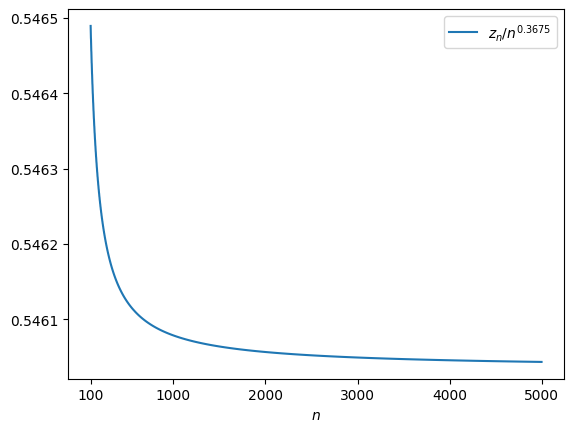
\includegraphics[width=\linewidth]{img/ratio-strict-lower-bound.png}
    \caption{Ratios $z_n/n^{\alpha}$ when $u = 0.5, v = 0.3$}
  \end{subfigure}
  \hfill
  \begin{subfigure}[c]{0.45\linewidth}
    \centering
    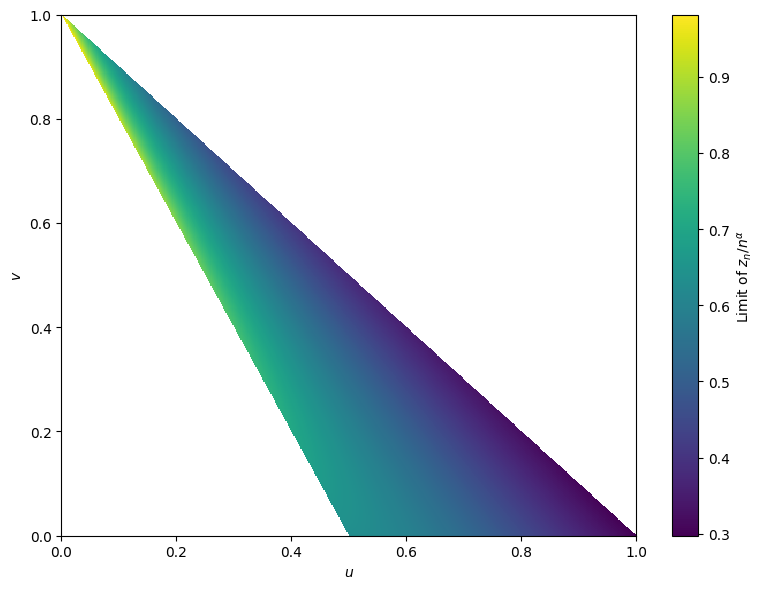
\includegraphics[width=\linewidth]{img/ratio-limits-strict-lower-bound.png}
    \caption{Limiting ratios for different $u$ and $v$.}
  \end{subfigure}

  \caption{Computation of $z_n/n^\alpha$}
  \label{fig:ratios}
\end{figure}


\begin{theorem}
  \label{thm:weaker-asymptotics}
  Let $\alpha$ be the solution to \eqref{eq:alpha-equation}. Then, $z_n = n^{\alpha + o(1)}$.
\end{theorem}

\begin{theorem}
  \label{thm:theta-asymptotics}
  Let $\alpha$ be the solution to \eqref{eq:alpha-equation}. Then, $z_n = \Theta(n^{\alpha})$.
\end{theorem}

For the exact asymptotics, we need to impose stricter conditions, for reasons that will become clear later.

\begin{equation}
  \label{eq:parameter-conditions-stronger}
  u,v \ge 0, \quad \dfrac{1}{2} < u < 1, \quad u+v\le1,
\end{equation}

\begin{theorem}
  \label{thm:exact-asymptotics}
  Let $(z_n)$ be defined by \eqref{eq:lower-bound-tighter}, let $\alpha$ be the solution to \eqref{eq:alpha-equation}, and let $u,v$ be the parameters satisfying \eqref{eq:parameter-conditions-stronger}. Then $z_n\sim C n^\alpha$ for some constant $C > 0$.
\end{theorem}

We begin with Theorem \ref{thm:weaker-asymptotics}. Rewrite the recurrence in \eqref{eq:lower-bound-tighter} as

\begin{equation}
  \label{eq:lower-bound-tighter-rewritten}
  z_{n+2} = \dfrac{1}{n}\sum\limits_{i=1}^n F(z_i, z_{n+1-i}), \quad n \ge 1,
\end{equation}
where
\begin{equation}
  F(x,y) = u(x+y) + v\max(x,y), \quad x,y > 0.
\end{equation}

Keeping in mind the heuristic $z_n \sim Cn^\alpha$, we try to approximate the right-hand side of \eqref{eq:lower-bound-tighter-rewritten}.

\begin{lemma}
  \label{thm:asymptoics-of-history}
  For every $\alpha \in (0,1]$, we have
  $$\dfrac{1}{n}\sum\limits_{i=1}^n F(i^\alpha, (n+1-i)^\alpha) \sim n^\alpha \Lambda(\alpha),$$
  where $\Lambda(\alpha) = \int_0^1 F(x^\alpha, (1-x)^\alpha) \,\mathrm{d}x = \dfrac{2(u+v)-v2^{-\alpha}}{\alpha+1}.$
\end{lemma}

\begin{proof}
  We will prove the equivalent limit
  $$\dfrac{1}{n}\sum\limits_{i=1}^n F\left(\left(\dfrac{i}{n}\right)^\alpha, \left(1-\dfrac{i}{n}+\dfrac{1}{n}\right)^\alpha\right) \to \Lambda(\alpha).$$

  Note that $\Lambda$ is continuous on $[0,1]$ with respect to $\alpha$, and the left-hand side is different from its Riemann sum only by a perturbation $1/n$ in the second argument. We show that the perturbation is negligible. Define for $x\in [0,1]$ the functions
  $$f_n(x) = F\left(x^\alpha, \left(1-x+\dfrac{1}{n}\right)^\alpha\right) \text{ and } f(x) = F(x^\alpha, (1-x)^\alpha).$$
  For $a,b,c \ge 0$ and $\alpha \in (0,1]$, we have
  $$|\max(a,b) - \max(a,c)| \le |b-c| \text{ and }
    (a+b)^\alpha \le a^\alpha + b^\alpha.$$
  Hence,
  \begin{align*}
    \|f_n-f\|_\infty
     & \le \sup\limits_{x\in[0,1]}(u+v)\left(\left(1-x+\dfrac{1}{n}\right)^\alpha - (1-x)^\alpha\right) \le (u+v)\dfrac{1}{n^\alpha} \to 0.
  \end{align*}

  Therefore,
  $$\left|\dfrac{1}{n}\sum\limits_{i=1}^n f_n\left(\dfrac{i}{n}\right) - \dfrac{1}{n}\sum\limits_{i=1}^n f\left(\dfrac{i}{n}\right)\right| \le \|f_n-f\|_\infty \to 0.$$
\end{proof}

The unique value of $\alpha$ such that $\Lambda(\alpha) = 1$ is the solution to \eqref{eq:alpha-equation}. To see this, compute
\begin{align*}
   & \Lambda'(\alpha) = \dfrac{v2^{-\alpha}\ln 2}{\alpha+1} - \dfrac{2(u+v)-v2^{-\alpha}}{(\alpha+1)^2} = \dfrac{v2^{-\alpha}((\alpha+1)\ln 2 + 1) - 2(u+v)}{(\alpha+1)^2}, \\
   & (2^{-\alpha}((\alpha+1)\ln 2 + 1))' = -2^{-\alpha}(\alpha+1)\ln^2(2) < 0.
\end{align*}
This implies
$$(\alpha+1)^2\Lambda'(\alpha) < (\alpha+1)^2\Lambda'(0) = -(2u + (1-\ln 2)v) < 0.$$
Hence, $\Lambda$ is strictly decreasing. We also have $\Lambda(0) = 2u+v > 1$ and $\Lambda(1) = u+v/2 < 1$. We exploit the fact that $\Lambda(\beta) > 1$ for $\beta < \alpha$ and $\Lambda(\beta) < 1$ for $\beta > \alpha$ to prove Theorem \ref{thm:weaker-asymptotics}.

\begin{proof}[Proof of Theorem \ref{thm:weaker-asymptotics}]
  Let $A_n(\beta) = \dfrac{1}{n}\sum\limits_{i=1}^n F(i^\beta, (n+1-i)^\beta)$. For the upper bound, let $\beta \in (\alpha, 1]$. Then $\Lambda(\beta) < 1$. Hence there exists $N$ such that for all $n \ge N$,
  $$A_n(\beta) < n^\beta < (n+2)^\beta.$$
  Let $M_n = \max_{1\le k \le n} \dfrac{z_i}{k^\beta}$. For $n \ge N$, we have
  $$z_{n+2} = \dfrac{1}{n}\sum_{i=1}^n F\left(z_i, z_{n+1-i}\right) \le M_n A_n(\beta) < M_n (n+2)^\beta.$$
  Hence, $\dfrac{z_{n+2}}{(n+2)^\beta} < M_n$. Thus $(M_n)$ is eventually decreasing, and $z_n = O(n^\beta)$.

  A similar argument applies for the lower bound, with an adjustment to deal with $z_2$. We have
  $$A_n(\beta) \sim n^\beta \sim (n+2)^\beta \text{ and } A_n(\beta) \sim \dfrac{1}{n}\sum\limits_{i=3}^{n-2} F(i^\beta, (n+1-i)^\beta).$$
  Assume that $\beta < \alpha$. Then, $\Lambda(\beta) > 1$. Hence there exists $N\ge 3$ such that for all $n \ge N$,
  $$\dfrac{1}{n}\sum\limits_{i=3}^{n-2} F(i^\beta, (n+1-i)^\beta) > (n+2)^\beta.$$
  Let $m_n = \min_{3\le i \le n-2} \dfrac{z_i}{i^\beta}$. For $n \ge N$, we have
  $$z_{n+2} \ge \dfrac{1}{n}\sum_{i=3}^{n-2} F\left(z_i, z_{n+1-i}\right) \ge m_n \dfrac{1}{n}\sum\limits_{i=3}^{n-2} F(i^\beta, (n+1-i)^\beta) > m_n (n+2)^\beta.$$
  Hence, $\dfrac{z_{n+2}}{(n+2)^\beta} > m_n$. Thus $(m_n)$ is eventually increasing, and $z_n = \Omega(n^\beta)$.
\end{proof}

The proof of Theorem \ref{thm:theta-asymptotics} uses a fine-grained induction. We first prepare integral bounds for the sum of the maximum terms.

\begin{lemma}
  \label{lem:integral-bounds}
  Let $f: [0, \infty) \to \mathbb{R}$ be an increasing function. For every integer $n \ge 1$, we have
  $$S_1 := \sum_{i=0}^{n-1} \max(f(i), f(n-1-i)) \le 2\int_{n/2}^n f(x) \, \mathrm{d}x \le S_2 :=\sum_{i=1}^{n} \max(f(i), f(n+1-i)). $$
\end{lemma}

\begin{proof}
  We first prove the upper bound on the first sum. We will use the following bounds for $t\ge 0$:
  $$f(t) \le \int_{t}^{t+1} f(x) \, \mathrm{d}x \le 2 \int_{t+1/2}^{t+1} f(x) \, \mathrm{d}x.$$

  If $n=2k$, we have
  $$S_1 = 2 \sum_{i=k}^{2k-1} f(i) \le 2 \sum_{i=k}^{2k-1} \int_{i}^{i+1} f(x) \, \mathrm{d}x.$$
  If $n=2k+1$, we have
  $$ S_1 = 2 \sum_{i=k+1}^{2k} f(i) + f(k) \le 2 \sum_{i=k+1}^{2k} \int_i^{i+1} f(x) \, \mathrm{d}x + 2 \int_{k+1/2}^{k+1} f(x) \, \mathrm{d}x.$$

  The lower bound on the second sum follows analogously from the following estimates. For $t\ge 1$, we have
  $$f(t) \ge \int_{t-1}^{t} f(x) \, \mathrm{d}x \ge 2 \int_{t-1}^{t-1/2} f(x) \, \mathrm{d}x.$$
\end{proof}


\begin{proof}[Proof of Theorem \ref{thm:theta-asymptotics}]
  We prove the lower bound. First, $z_n > 0$ for all $n\ne 2$. The main idea is to isolate $z_2$. The induction hypothesis is $z_n \ge K (n+L)^\alpha$ for $n\neq 2$. The base cases and the exact constants are determined later. We need
  $$\max(z_2, z_{n-1})= z_{n-1} \ge \max((2+L)^\alpha, (n-1+L)^\alpha).$$
  Thus, for $n \ge 3$,
  \begin{align*}
    nz_{n+2}
     & = 2u\sum\limits_{i=1}^n z_i + v\sum\limits_{i=1}^n \max(z_i, z_{n+1-i})                                                                \\
     & \ge K\left(2u\sum\limits_{i=1}^{n} (i+L)^\alpha + v\sum\limits_{i=1}^{n} \max((i+L)^\alpha, (n+1-i+L)^\alpha)\right) - K2u(2+L)^\alpha \\
     & \ge K\left(2u\int_0^{n} (x+L)^\alpha \, \mathrm{d}x + 2v\int_{n/2}^{n} (x+L)^\alpha \, \mathrm{d}x\right) - K2u(2+L)^\alpha.
  \end{align*}
  Let
  \begin{align*}
    A_n
     & = 2u\int_0^{n} (x+L)^\alpha \, \mathrm{d}x + 2v\int_{n/2}^{n} (x+L)^\alpha \, \mathrm{d}x             \\
     & = \dfrac{1}{\alpha+1}\left((2u+2v)(n+L)^{\alpha+1} - 2v\left(\dfrac{n}{2}+L\right)^{\alpha+1}\right).
  \end{align*}
  Using the expansions
  \begin{align*}
    (n+L)^{\alpha+1}                       & = n^{\alpha+1} + (\alpha+1)L n^\alpha + O(n^{\alpha-1}),                         \\
    \left(\dfrac{n}{2}+L\right)^{\alpha+1} & = 2^{-\alpha+1}n^{\alpha+1} + (\alpha+1)L2^{-\alpha} n^\alpha + O(n^{\alpha-1}),
  \end{align*}
  we get
  \begin{align*}
    A_n
     & = n^{\alpha+1} + L(2u+2v-2v2^{-\alpha})n^\alpha + O(n^{\alpha-1})        \\
     & = n^{\alpha+1} + L(\alpha + 1 - v2^{-\alpha})n^\alpha + O(n^{\alpha-1}).
  \end{align*}
  On the other hand,
  $$n(n+L+2)^\alpha = n^{\alpha+1} + \alpha(L+2) n^\alpha + O(n^{\alpha-1}).$$
  Hence,
  $$A_n - 2u(2+L)^\alpha - n(n+L+2)^\alpha = (L(1-v2^{-\alpha}) - 2\alpha) n^\alpha + O(n^{\alpha-1}).$$
  Since $1-v2^{-\alpha} > 0$, choose $L>\dfrac{2\alpha}{1-v2^{-\alpha}}$, then there exists $N$ such that for all $n \ge N$,
  $$A_n - 2u(2+L)^\alpha - n(n+L+2)^\alpha \ge 0,$$
  implying that $z_{n+2} \ge K(n+L+2)^\alpha$. Finally, we choose
  $$K = \min\limits_{\substack{1\le i\le N+1 \\ i\ne 2}}\dfrac{z_i}{(i+L)^\alpha} > 0$$
  to satisfy the base cases $i\le N+1$, excluding $i=2$ where $z_2=0$. \pablo{the base cases $i\leq N+1$ where $N$ is chosen to satisfy the above inequality.}

  \pablo{$K$ below is not the same as above. Write e.g., $\tilde{K}$}

  We now prove the upper bound. Our induction hypothesis is $z_n \le \tilde{K} (n-1)^\alpha$ for $n\ge 2$, for some constant $\tilde{K} > 1$. The base case $z_2=0$ is trivially satisfied. For $n\ge 2$, we have
  \begin{align*}
    nz_{n+2}
     & = 2u + 2u\sum\limits_{i=2}^n z_i + v\sum\limits_{i=1}^n \max(z_i, z_{n+1-i})                                              \\
     & \le \tilde{K}\left(2u\sum\limits_{i=1}^{n-1} i^\alpha + v\sum\limits_{i=0}^{n-1} \max(i^\alpha, (n-1-i)^\alpha)\right)+2u \\
     & \le \tilde{K}\left(2u\int_1^{n} x^\alpha \, \mathrm{d}x + 2v\int_{n/2}^{n} x^\alpha \, \mathrm{d}x\right) + 2u            \\
     & = \tilde{K}\left(2u\dfrac{n^{\alpha+1} - 1}{\alpha+1} + 2v\dfrac{n^{\alpha+1} - (n/2)^{\alpha+1}}{\alpha+1}\right)+2u     \\
     & = \tilde{K}n^{\alpha+1}\dfrac{2u+2v - v2^{-\alpha}}{\alpha+1}- \dfrac{2\tilde{K}u}{\alpha+1}+2u                           \\
     & = \tilde{K}n^{\alpha+1} - \dfrac{2\tilde{K}u}{\alpha+1} + 2u.
  \end{align*}


  The first inequality is valid by noticing that
  $$\max(z_1, z_n) = \max(1, z_n) \le \tilde{K}(n-1)^\alpha = \tilde{K}\max(0, (n-1)^\alpha).$$
  The second inequality uses Lemma \ref{lem:integral-bounds}. Choose $\tilde{K}=\alpha+1 > 1$, then $z_{n+2} \le \tilde{K}n^\alpha \le \tilde{K}(n+2)^\alpha$.
\end{proof}

\begin{remark}
  In the proof of the lower bound, we use the fact that $(n+L)^{\alpha+1}$ dominates $n(n+L+2)^{\alpha+1}$ when $L$ is large enough. Similarly, $(n-L)^{\alpha+1} \ll n(n-L+2)^{\alpha+1}$ for large $L$. However, applying the same idea to the upper bound would start the induction only after some $n > L$. We avoid this by choosing $L=1$ and saving a fixed budget $2u$ in the first term, which also gives a useful algebraic simplification.
\end{remark}

We now prove the exact asymptotics stated in Theorem \ref{thm:exact-asymptotics}. A natural goal is to remove the maximum operator. If $z_1=z_2=1$, then the sequence would be increasing from the beginning, and induction would allow us to eliminate the maximum operator. However, the initial conditions $z_1=1$ and $z_2=0$ make the sequence $(z_n)$ fluctuate during the first iterations, and the index at which it becomes increasing depends on the parameters $u$ and $v$. An extreme case of a long fluctuation period occurs when $u\to1/2+$ and $v\to0+$. We illustrate this phenomenon and compare the two cases in Figure~\ref{fig:difference-beginning}. The figure compares the consecutive differences of the same recurrence under two close initializations, $z_1=z_2=1$ and $z_1=1,z_2=0$, in the difficult regime $u=0.5000001$ and $v=0.000001$. The second initialization can create a long initial fluctuation, which explains why monotonicity cannot simply be assumed from the beginning.

\begin{figure}
  \begin{subfigure}[c]{0.45\linewidth}
    \centering
    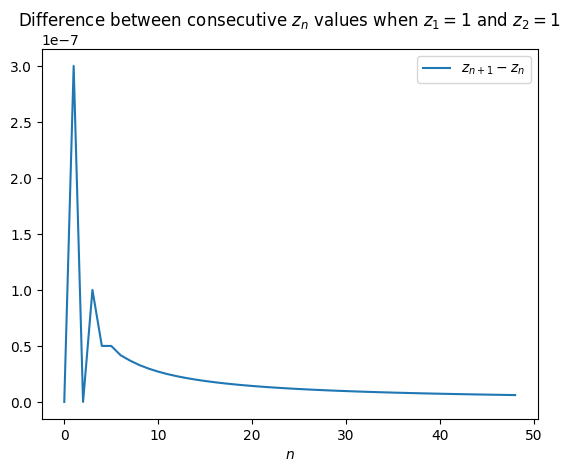
\includegraphics[width=\linewidth]{img/strict-lower-bound-11.png}
  \end{subfigure}
  \hfill
  \begin{subfigure}[c]{0.45\linewidth}
    \centering
    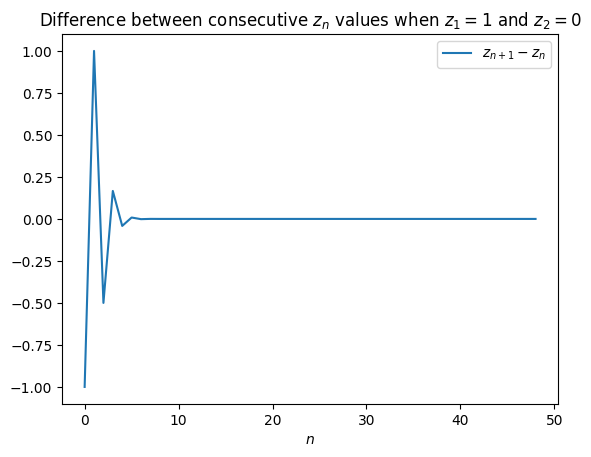
\includegraphics[width=\linewidth]{img/strict-lower-bound-10.png}
  \end{subfigure}

  \caption{First consecutive differences of $(z_n)$ in two initializations ($u = 0.5000001, v = 0.000001$)}
  \label{fig:difference-beginning}
\end{figure}

\pablo{Give experimental examples.}



Eventual monotonicity is sufficient to remove the maximum operator. Assume that there exists $N_1$ such that $z_{n+1} \ge z_n$ for all $n \ge N_1$. Since $(z_n)$ is unbounded, there exists $N_2 \ge N_1$ such that for all $n \ge N_2$, we have both $z_{n+1} \ge \max\limits_{1\le i \le N_1} z_i$ and $z_{n+1} \ge z_n$. That is,
$$\forall n \ge N_2, \quad z_{n+1} \ge \max_{1 \le i \le n} z_i.$$
Taking $N_3 = 2N_2-1$, we have \cyril{the writing $\forall \dfrac{N_3+1}{2}\le i \le N_3$ looks weird}
$$\forall n \ge N_3,\quad \forall i\in\left\{\left\lceil\dfrac{n+1}{2}\right\rceil,\ldots,n\right\}, \quad z_{i} \ge z_{n+1-i}.$$

Under the stronger parameter condition \eqref{eq:parameter-conditions-stronger}, Theorem~\ref{thm:eventually-increasing} below proves that such an index exists. The question about the first index where the fluctuations stop is itself interesting, and we leave it open.
\begin{openquestion}
  \label{open:when-eventually-increasing}
  In terms of $u$ and $v$, what is the first index $N$ such that $(z_n)_{n\ge N}$ is increasing?
\end{openquestion}


\pablo{The existence of $N$  is Theorem~\ref{thm:eventually-increasing}, right ? You can announce the results, otherwise one might think that the existence of $N$ is conjectured.}

We proceed to proving eventual monotonicity. The idea is to use loose inequalities to bootstrap basic properties, then upgrade step by step with tighter inequalities. The next lemma uses a loose inequality $\max(a,b)\le a+b$ to show that the difference between consecutive terms vanishes. To begin with, let us define for $n\ge 1$ the difference
$$\Delta z_n = z_{n} - z_{n-1}.$$

\begin{lemma}[Vanishing difference]
  \label{lem:vanishing-difference}
  We have $|\Delta z_n| \to 0$.
\end{lemma}

\begin{proof}
  For $n \ge 2$, we have
  \begin{align*}
    nz_{n+2}     & = 2u\sum_{i=1}^n z_i + v\sum_{i=1}^n \max(z_i, z_{n+1-i}),       \\
    (n-1)z_{n+1} & = 2u\sum_{i=1}^{n-1} z_i + v\sum_{i=1}^{n-1} \max(z_i, z_{n-i}).
  \end{align*}
  Subtracting the equations side by side, we get
  \begin{equation}
    \label{eq:difference}
    \begin{aligned}
      n\Delta z_{n+2}
       & = 2uz_n + v\max(z_n,z_1) - z_{n+1} + v\sum_{i=1}^{n-1} (\max(z_i, z_{n+1-i}) - \max(z_i, z_{n-i}))      \\
       & = 2uz_n + v\max(z_n,z_1) - z_{n+1} + v\sum_{i=1}^{n-1} (\max(z_{n-i}, z_{i+1}) - \max(z_{n-i}, z_{i})).
    \end{aligned}
  \end{equation}
  Using $\max(z_n, z_1) \le z_n+z_1$, we have
  \begin{align*}
    n\Delta z_{n+2}
     & \le 2uz_n + v(z_n + z_1) - vz_{n+1} + v\sum_{i=1}^{n-1} (\max(z_{n-i}, z_{i+1}) - \max(z_{n-i}, z_{i})) \\
     & \le 2uz_n + vz_1 + v(z_n - z_{n+1}) + v\sum_{i=1}^{n-1} (\max(z_{n-i}, z_{i+1}) - \max(z_{n-i}, z_{i}))
  \end{align*}
  Using $|\max(a,b) - \max(a,c)| \le |b-c|$, we have
  \begin{align*}
    n|\Delta z_{n+2}|
     & \le 2uz_n + vz_1 + v|\Delta z_n| + v\sum_{i=1}^{n-1} |\Delta z_i| = 2uz_n + vz_1 + v\sum_{i=1}^{n}|\Delta z_i| \\
     & \le 2uz_n + vz_1 + nv\sup_{1\le i \le n}|\Delta z_i|.
  \end{align*}
  Since $u < 1$, we have $\alpha < 1$. By $z_n = \Theta(n^\alpha)$, we have $\dfrac{1}{n}(2uz_n + vz_1) \to 0$, or
  $$|\Delta z_{n+2}| \le v\sup_{1\le i \le n}|\Delta z_i| + o(1).$$
  We have $v < 1$ since otherwise the condition $2u+v > 1$ would be violated. Therefore $(|\Delta z_i|)$ is bounded. Let $M = \sup_{n \ge 1} |\Delta z_n|$. For every $\epsilon > 0$, there exists $N$ such that for all $n \ge N$, $|\Delta z_n| < M + \epsilon$. Therefore,
  $$|\Delta z_{n+2}| \le v(M+\epsilon) + o(1).$$
  Letting $n\to\infty$ gives $M \le v(M+\epsilon)$. Since $\epsilon > 0$ is arbitrary, we have $M = 0$.
\end{proof}

Since $(z_n)$ is unbounded, we have the following corollary.

\begin{corollary}[Eventual exceedance]
  \label{cor:eventual-exceed}
  Let $\alpha$ be the solution to \eqref{eq:alpha-equation}. Then, for every $M > 0$, there exists $N$ such that for all $n \ge N$, $z_n > M$.
\end{corollary}

\begin{lemma}[Difference identity]
  \label{lem:difference-identity}
  For all sufficiently large $n$, there exist numbers $\theta_{n,i}\in [0,1]$ for $1\le i\le n-1$ such that
  \begin{equation}
    \label{eq:difference-identity}
    n\Delta z_{n+2} = (2u+v-1)z_n-\Delta z_n +v\sum_{i=1}^{n-1}\theta_{n,i}\Delta z_i.
  \end{equation}
\end{lemma}

\begin{proof}
  We start from \eqref{eq:difference}
  $$n\Delta z_{n+2} = 2uz_n + v\max(z_n,z_1) - z_{n+2} + v\sum_{i=1}^{n-1} (\max(z_i, z_{n+2-i}) - \max(z_i, z_{n-i})).$$
  By Corollary \ref{cor:eventual-exceed}, we have $\max(z_n,z_1)=z_n$ for all sufficiently large $n$. Hence, for all sufficiently large $n$,
  $$n\Delta z_{n+2} = (2u+v-1)z_n -\Delta z_n + v\sum_{i=1}^{n-1} (\max(z_{n-i}, z_{i+2}) - \max(z_{n-i}, z_{i})).$$
  For every $a \ge 0$, the function $x\mapsto \max(a,x)$ is increasing and $1$-Lipschitz. Hence for each $n,i$ there is some $\theta_{n,i}\in[0,1]$ satisfying \eqref{eq:difference-identity}.
\end{proof}

At this step, we have isolated the difference sequence $(\Delta z_n)$ from the original sequence $(z_n)$. Our next goal is to prove that $(\Delta z_n)$ is \textit{eventually positive}. This would follow if, in \eqref{eq:difference-identity}, a lower bound for $-\Delta z_n + v\sum_{i=1}^{n-1}\theta_{n,i}\Delta z_i$ could be absorbed into $(2u+v-1)z_n$. We already have $|\Delta z_n| = o(z_n)$ since $(\Delta z_n)$ is bounded.

Because little is known about $\theta_{n,i}$, we can only use a worst-case bound. A basic absolute-value estimate would require proving that $\sum_{i=1}^{n}|\Delta z_i| = o(z_n)$. However, if $z_n\sim Cn^\alpha$ and $z_n$ is eventually increasing, then $\sum_{i=1}^{n}|\Delta z_i| \sim Cn^\alpha$. We therefore need a tighter lower bound. We use the \textit{negative variation} of $\Delta z_n$, defined for every $x\in\mathbb{R}$ as
\begin{equation}
  x_{-} = \max(-x,0).
\end{equation}

We have
\begin{equation}
  \label{ineq:negative-variation}
  -x \le x_{-} \text{ and } 0 \le x_{-}.
\end{equation}

Define the negative variation series of $(\Delta z_n)$ as
\begin{equation}
  \label{eq:negative-variation}
  V_n := \sum_{i=1}^{n} (\Delta z_i)_{-}.
\end{equation}
Then $(V_n)$ is increasing. We state the criterion for eventual increase of $(z_n)$ in terms of $(V_n)$ as follows.

\begin{lemma}[Negative variation criterion]
  If $V_n = o(z_n)$, then $(z_n)$ is eventually increasing.
\end{lemma}

\begin{proof}
  By Lemma~\ref{lem:difference-identity}, for all sufficiently large $n$,
  $$n\Delta z_{n+2} \ge (2u+v-1)z_n-|\Delta z_n|-vV_n.$$
  Since $\Delta z_n$ is bounded and $z_n\to\infty$, we have $|\Delta z_n|=o(z_n)$. By assumption, $V_n = o(z_n)$. Hence for all sufficiently large $n$,
  $$n\Delta z_{n+2} \ge \dfrac{1}{2}(2u+v-1)z_n > 0$$
\end{proof}

% It would be perfect if we could prove that $(V_n)$ is bounded, as this is indeed the truth. However, it is already good to prove that $V_n = o(n^\alpha)$, since we already have $z_n = \Theta(n^\alpha)$.

\pablo{``probably'' or ``likely' ' rather than ``indeed''}

Numerical experiments suggest that $(V_n)$ is likely bounded. For the proof of eventual monotonicity, however, the following weaker estimate is enough.

\begin{lemma}
  Assume that $v>0$.
  We have $V_n = O(n^v)$.
\end{lemma}

\begin{proof}
  Again, we start from \eqref{eq:difference-identity}. There exists $N$ such that for all $n\ge N$,
  $$n\Delta z_{n+2} = (2u+v-1)z_n - \Delta z_n + v\sum_{j=1}^{n-1}\theta_{n,j}\Delta z_j.$$
  Let $M = \sup |\Delta z_n|$. \pablo{You mean $\Delta z_n$. Also, I am not convinced of the next equality. You do have the inequality with $v \sum (\Delta z_j)_-$, but not an equality as it is not true that $(x+y)_-=x_-+y_-$}
  If $\Delta z_{n+2}\ge 0$, then $(\Delta z_{n+2})_- = 0$. Otherwise, $(\Delta z_{n+2})_- = -\Delta z_{n+2}$, and therefore
  \begin{align*}
    n(\Delta z_{n+2})_-
     & = \Delta z_n - (2u+v-1)z_n - v\sum_{j=1}^{n-1}\theta_{n,j}\Delta z_j                                                       \\
     & \le |\Delta z_n| - (2u+v-1)z_n + v\sum_{j=1}^{n-1}\theta_{n,j}(\Delta z_j)_- & (- \Delta z_j\le (\Delta z_j)_-, \forall j) \\
     & \le |\Delta z_n| + v\sum_{j=1}^{n-1}(\Delta z_j)_-                           & (0\le\theta_{n,j}\le1)                      \\
     & \le M + vV_{n-1}.
  \end{align*}
  Thus, in either case,
  $$(\Delta z_{n+2})_- \le \dfrac{v}{n}V_{n-1}+\dfrac{M}{n}.$$
  Since $(V_n)$ is increasing, we get
  \begin{equation}
    \label{eq:negative-variation-bound}
    V_{n+2}
    = V_{n+1}+(\Delta z_{n+2})_-
    \le \left(1+\dfrac{v}{n}\right)V_{n+1}+\dfrac{M}{n}.
  \end{equation}
  Reindexing, for every $m\ge N+2$,
  $$V_m + \dfrac{M}{v} \le \left(1+\dfrac{v}{m-2}\right)\left(V_{m-1} + \dfrac{M}{v}\right).$$
  Iterating this inequality gives
  $$V_m + \dfrac{M}{v}
    \le \prod_{i=N}^{m-2}\left(1+\dfrac{v}{i}\right)\left(V_{N+1} + \dfrac{M}{v}\right).$$
  It remains to estimate the product. Taking the logarithm gives
  \begin{align*}
    \ln\left(\prod_{i=N}^{m-2}\left(1+\frac{v}{i}\right) \right)
     & = \sum_{i=N}^{m-2}\ln\left(1+\frac{v}{i}\right)         \\
     & \le \sum_{i=N}^{m-2} \frac{v}{i} = v(H_{m-2} - H_{N-1}) \\
     & \le vH_m \le v\ln m + C,
  \end{align*}
  where $H_n=\sum_{i=1}^n \frac{1}{i} = \ln n + \gamma + O(1/n)$ is the $n$-th harmonic number and $C$ is some constant. Exponentiating both sides yields
  $$\prod_{i=N}^{m-2} \left( 1 + \frac{v}{i} \right) \le e^{C} m^v = O(m^v).$$
\end{proof}

We state our checkpoint as a theorem.

\begin{theorem}
  \label{thm:eventually-increasing}
  If $0<v < \alpha$, then $(z_n)$ is eventually increasing.
\end{theorem}

\begin{proof}
  By the previous lemma, $V_n=O(n^v)=o(n^\alpha)=o(z_n)$, since $v<\alpha$ and $z_n=\Theta(n^\alpha)$. The result follows from the negative variation criterion.
\end{proof}

When $v=0$, the recurrence \eqref{eq:lower-bound-tighter} reduces to the full-history recurrence \eqref{eq:lower-bound}, whose asymptotics are handled by Proposition~\ref{lem:full-history-sum-asymptotics}. Thus the negative-variation argument is only needed for $v>0$.

We now express the condition $0<v < \alpha$ in terms of $u$ and $v$. Define
$$f(\alpha) = \alpha + 1 - 2(u + v) + v 2^{-\alpha}, \alpha\in[0,1].$$
Then $f'(\alpha) = 1 - v2^{-\alpha}\ln2 > 1-\ln2 > 0$ for all $\alpha > 0$. Hence $v < \alpha$ is equivalent to $f(v) < 0$ i.e.,
$$v + 1 - 2(u + v) + v 2^{-v} < 0 \iff u > \frac{1}{2}(1 - v + v 2^{-v}).$$
For $v>0$, if we impose conditions \eqref{eq:parameter-conditions-stronger}, then the above inequality is satisfied. The case $v\ge \alpha$ with $v>0$ is left open. Once $(z_n)$ is eventually increasing, it satisfies a simpler recurrence without the whole history.

\begin{lemma}
  There exists $N\ge 1$ such that the sequence $(z_n)_{n\ge N}$ defined by \ref{eq:lower-bound-tighter} satisfies the recurrence
  \begin{equation}
    \label{eq:delayed-recurrence}
    nz_{n+2}-(n-1)z_{n+1} = 2(u+v)z_{n} - vz_{\lfloor n/2\rfloor}.
  \end{equation}
  with $z_{N+1} \ge z_{N} \ge \ldots \ge z_{\lfloor n/2\rfloor} \ge 1$.
\end{lemma}

\begin{proof}
  Since $(z_n)$ is eventually increasing, there exists $N$ such that for all $n\ge N$, we have $z_n \ge z_i$ for all $1\le i \le n-1$ and $z_n \ge 1$. Hence, for all $n\ge N+1$,
  \begin{align*}
    nz_{n+2}     & = 2u\sum_{i=1}^n z_i + 2v\sum_{i=\lceil n/2\rceil+1}^n z_i + \delta_nvz_{\lceil n/2\rceil}                      \\
    (n-1)z_{n+1} & = 2u\sum_{i=1}^{n-1} z_i + 2v\sum_{i=\lceil (n-1)/2\rceil+1}^{n-1} z_i + \delta_{n-1}vz_{\lceil (n-1)/2\rceil},
  \end{align*}
  where $\delta_n = 1$ if $n$ is odd and $0$ if $n$ is even. If $n=2k$, then $\lceil n/2\rceil = \lceil (n-1)/2\rceil = k$, $\delta_n = 0$ and $\delta_{n-1} = 1$. Hence,
  $$2kz_{2k+2} - (2k-1)z_{2k+1} = 2(u+v)z_{2k} - vz_{k}.$$
  If $n=2k+1$, then $\lceil n/2\rceil > \lceil (n-1)/2\rceil = k$, $\delta_n = 1$ and $\delta_{n-1} = 0$. Hence,
  $$(2k+1)z_{2k+3} - (2k)z_{2k+2} = 2(u+v)z_{2k+1} - 2vz_{k+1} + vz_{k+1} = (2k+1)(u+v)z_{2k+1} - vz_{k+1}.$$
  Collecting the two cases and noticing that $\left\lceil\dfrac{n-1}{2}\right\rceil = \left\lfloor\dfrac{n}{2}\right\rfloor$, we arrive at \eqref{eq:delayed-recurrence}.
\end{proof}

With the recurrence \eqref{eq:delayed-recurrence}, we can now prove the exact asymptotics of $(z_n)$. We will use a dyadic argument to show that the normalized difference sequence $(\Delta x_n)$ is absolutely summable by analyzing it on the intervals $[2^m, 2^{m+1})$.

        \pablo{You can pre-state this result at the beginning of the chapter to outline it, citing it forward.}

        \begin{proof}[Proof of Theorem~\ref{thm:exact-asymptotics}]
          Let $x_n=\dfrac{z_n}{(n-2)^\alpha}$ for $n\ge N$. We will prove that $(x_n)$ converges by proving that $(\Delta x_n)$ is absolutely summable, i.e., $\sum_{n\ge N}|\Delta x_n|$ converges. Note that $x_n = \Theta(1)$ since $z_n = \Theta(n^\alpha)$. For $n\ge N \ge 6$ (so that $x_{\lfloor n/2\rfloor}$ is defined), we have
          \begin{align*}
                 & n^{\alpha+1} x_{n+2} - (n-1)^{\alpha+1} x_{n+1} = 2(u+v)(n-2)^{\alpha}x_{n} - v\left(\left\lfloor \dfrac{n}{2}\right\rfloor-2\right)^{\alpha}x_{\lfloor n/2\rfloor}                                               \\
            \iff & x_{n+2} = \left(1-\dfrac{1}{n}\right)^{\alpha+1}x_{n+1} + \dfrac{2(u+v)}{n}\left(1-\dfrac{2}{n}\right)^{\alpha}x_{n-1} - \dfrac{v}{n}\left(\dfrac{\lfloor n/2\rfloor-2}{n}\right)^{\alpha}x_{\lfloor n/2\rfloor}.
          \end{align*}
          We have
          \begin{align*}
             & \left(1-\dfrac{1}{n}\right)^{\alpha+1} = 1 - \dfrac{\alpha+1}{n} + O\left(\dfrac{1}{n^2}\right),                        \\
             & \dfrac{1}{n}\left(1-\dfrac{2}{n}\right)^{\alpha} = \dfrac{1}{n} + O\left(\dfrac{1}{n^2}\right),                         \\
             & \frac{1}{n}\left(\dfrac{\lfloor n/2\rfloor-2}{n}\right)^{\alpha} = \frac{2^{-\alpha}}{n} + O\left(\frac{1}{n^2}\right).
          \end{align*}
          The last expansion follows from $\dfrac{1}{2}-\dfrac{3}{n} \le \dfrac{\lfloor n/2\rfloor-2}{n} \le \dfrac{1}{2}-\dfrac{1}{n}$. Since $\alpha$ solves \eqref{eq:alpha-equation}, we have
          \begin{align*}
            x_{n+2}-x_{n+1}
             & = -\dfrac{\alpha+1}{n}x_{n+1} + \dfrac{2(u+v)}{n}x_{n} - \frac{v2^{-\alpha}}{n}x_{\lfloor n/2\rfloor} + O\left(\frac{1}{n^2}\right)   \\
             & = -\dfrac{2(u+v)}{n}(x_{n+1}-x_{n}) + \frac{v2^{-\alpha}}{n}\left(x_{n}- x_{\lfloor n/2\rfloor}\right) + O\left(\frac{1}{n^2}\right).
          \end{align*}

          There exists a constant $K_1>0$ such that for every $n\ge N'-2 \ge N$,
          $$|\Delta x_{n+2}| \le \dfrac{2(u+v)}{n}|\Delta x_{n+1}| + \frac{v2^{-\alpha}}{n}\sum_{i=\lfloor n/2\rfloor + 1}^{n}|\Delta x_{i}| + \dfrac{K_1}{(n+2)^2}.$$
          Equivalently, for $n\ge N'$,
          $$|\Delta x_{n}| \le \dfrac{2(u+v)}{n-2}|\Delta x_{n-1}| + \frac{v2^{-\alpha}}{n-2}\sum_{i=\lfloor n/2\rfloor}^{n-2}|\Delta x_{i}| + \dfrac{K_1}{n^2}.$$

          Let $u_m = \max_{2^m \le n < 2^{m+1}} |\Delta x_n|$. Then, for every $n\in [2^m, 2^{m+1})$, we have
          \begin{align*}
             & |\Delta x_{n-1}| \le \max_{2^m-1\le i < 2^{m+1}-1}|\Delta x_i| \le \max(u_{m-1},u_m),                                                                             \\
             & \dfrac{1}{n-2}\sum_{i=\lfloor n/2\rfloor}^{n-2}|\Delta x_{i}| \le \dfrac{1}{2}\max_{2^{m-1}\le i < 2^{m+1}-2} |\Delta x_i|\le  \dfrac{1}{2} \max(u_{m-1}, u_{m}).
          \end{align*}
          Therefore,
          \begin{align*}
            |\Delta x_{n}|
             & \le \left(\dfrac{2(u+v)}{n-2}+v2^{-\alpha-1}\right)\max(u_{m-1},u_m) + \dfrac{K_1}{2^{2m}}.
          \end{align*}
          Taking the maximum over $n\in [2^m, 2^{m+1})$, we have
          \begin{align*}
            u_m
             & \le \left(\dfrac{2(u+v)}{n-2}+v2^{-\alpha-1}\right)\max(u_{m-1},u_m) + \dfrac{K_1}{2^{2m}}.
          \end{align*}
          Since $v2^{-\alpha} = 2(u+v)-\alpha-1 < 1$, we can choose $m_0$ large enough such that $2^{m_0} \ge N'$, and there exists $\gamma_1$ such that
          $$\dfrac{2(u+v)}{n-2}+ v2^{-\alpha-1} < \gamma_1 < \dfrac{1}{2}$$
          for all $m\ge m_0$ and $n\in [2^m, 2^{m+1})$. If $u_{m-1} > u_m$, then $u_m \le \gamma_1 u_{m-1} + \dfrac{K_1}{2^{2m}}$. If $u_{m-1} \le u_m$, then $u_m \le \dfrac{K_1}{2^{2m}(1-\gamma_1)}$. In both cases, we have
          \begin{align*}
            u_m
             & \le \gamma_1 u_{m-1} + \dfrac{K_1}{2^{2m}(1-\gamma_1)}                                                             \\
             & \le \sum_{i=m_0+1}^m \gamma_1^{m-i}\dfrac{K_1}{2^{2i}(1-\gamma_1)} + \gamma_1^{m-m_0}u_{m_0}                       \\
             & < \dfrac{K_1}{(1-\gamma_1)}\sum_{i=m_0+1}^m \gamma_1^{m-i}\left(\dfrac{1}{4}\right)^{i} + \gamma_1^{m-m_0}u_{m_0}.
          \end{align*}
          Choose $\gamma_2$ such that $\max\left(\gamma_1, \dfrac{1}{4}\right) < \gamma_2 < \dfrac{1}{2}$. We have
          \begin{align*}
            u_m < \dfrac{K_1}{(1-\gamma_1)}\sum_{i=m_0+1}^m \gamma_2^m + \gamma_2^{m-m_0}u_{m_0} \le K_2 m\gamma_2^m,
          \end{align*}
          for some constant $K_2>0$. Choose $\gamma_3$ such that $\gamma_2 < \gamma_3 < \dfrac{1}{2}$. Then there exists $m_1>m_0$ such that for every $m\ge m_1$, we have $K_2m\gamma_2^m < K_2\gamma_3^m$, implying that
          $$u_m < K_2\gamma_3^m.$$
          Therefore,
          \begin{align*}
            \sum_{n=N'+1}^\infty|\Delta x_{m}|
             & \le \sum_{m=\lfloor\log_2(N')\rfloor}^\infty \sum_{n=2^m}^{2^{m+1}-1}|\Delta x_n| < \sum_{m=\lfloor\log_2(N')\rfloor}^{m_1-1} 2^m u_m  + K_2\sum_{m=m_1}^\infty (2\gamma_3)^{m} < \infty.
          \end{align*}
          Hence, $(x_n)$ converges to some constant $C>0$. Thus, $z_n \sim Cn^\alpha$.
        \end{proof}

        \section{Asymptotics of the stochastic recurrence}

        \subsection{Proof strategy}

        The stochastic recurrence \eqref{eq:longest-literal-recurrence} resembles its deterministic counterpart \eqref{eq:lower-bound-tighter}. Since \eqref{eq:lower-bound-tighter} grows as a pure power of $n$, it is natural to conjecture the same behavior for the expectation in \eqref{eq:expected-longest-literal-recurrence}. Numerical experiments based on Monte Carlo simulation support this conjecture, as shown in Figure \ref{fig:growth-comparison}. For each case of $(u,v)$, we compute the exponent $\alpha$ using the algorithm expressed in \eqref{eq:mean-preserving-recurrence}, and the constant $C=z_n/n^\alpha$, where $n$ is the number of iterations. More details of the algorithm are given later in this section.

        The growth exponent of $y_n$ is strictly larger than the solution to \eqref{eq:alpha-equation}. This suggests that, in the long term, $\EE\left[\max(Y_i, Y_j)\right]$ remains more selective than $\max(\EE[Y_i], \EE[Y_j])$, especially when $i$ and $j$ are close to each other.

        \begin{figure}
          \begin{subfigure}[c]{0.45\linewidth}
            \centering
            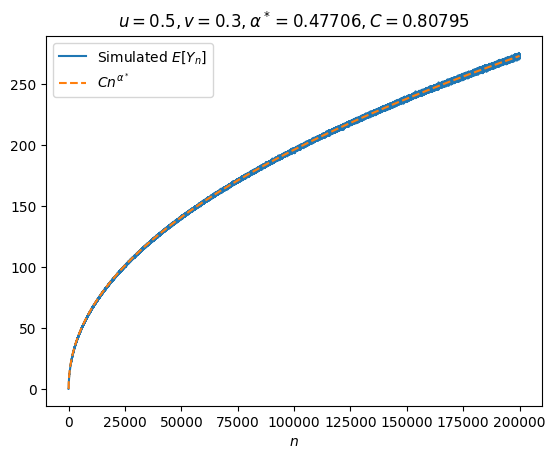
\includegraphics[width=\linewidth]{img/05-03-100000-200000.png}
          \end{subfigure}
          \hfill
          \begin{subfigure}[c]{0.45\linewidth}
            \centering
            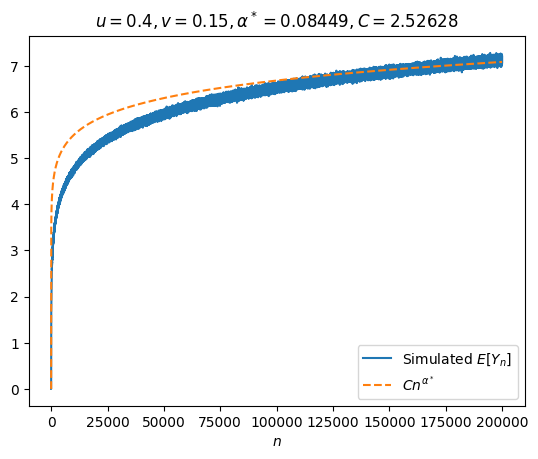
\includegraphics[width=\linewidth]{img/04-015-100000-200000.png}
          \end{subfigure}

          \caption{The growth of $y_n$ compared with a power $Cn^\alpha$}
          \label{fig:growth-comparison}
        \end{figure}


        In this section, we present an ongoing attempt to prove the weakest asymptotic result $y_n = n^{\alpha^\star + o(1)}$. We adapt the contraction method (e.g., \cite{neininger2004general}). The original idea is as follows.
        \begin{enumerate}
          \item Guess the scaling factor and derive the normalized recurrence.
          \item Derive a limiting fixed-point equation from the normalized recurrence.
          \item Prove that the limiting equation has a unique solution in a suitable metric space using a contraction argument.
          \item Prove that the normalized sequence converges in distribution to that unique solution.
        \end{enumerate}

        We first explain why the contraction method does not apply directly. Let $X_n = Y_n/n^\alpha$ for $\alpha > 0$. The recurrence for $X_n$ and the limiting equation are as follows.

        \begin{equation}
          \label{eq:scaled-recurrence}
          \begin{aligned}
            X_{n+2}
             & \stackrel{d}{=} I\left(\left(\dfrac{U_n}{n+2}\right)^\alpha X_{U_n}^{(1)} + \left(\dfrac{n+1-U_n}{n+2}\right)^\alpha X_{n+1-U_n}^{(2)}\right)   \\
             & \myspace{50} + J\max\left(\left(\dfrac{U_n}{n+2}\right)^\alpha X_{U_n}^{(1)}, \left(\dfrac{n+1-U_n}{n+2}\right)^\alpha X_{n+1-U_n}^{(2)}\right)
          \end{aligned}
        \end{equation}

        \begin{lemma}[Limiting equation]
          \label{lem:limiting-equation}
          Suppose that $X_n \stackrel{d}{\to} X$. Then, $X$ satisfies the following distributional equation
          \begin{equation}
            \label{eq:limiting-equation}
            X \stackrel{d}{=} I\left(U^\alpha X^{(1)} + (1-U)^\alpha X^{(2)}\right) + J\max(U^\alpha X^{(1)}, (1-U)^\alpha X^{(2)}),
          \end{equation}
          where $U \sim \mathrm{Unif}[0,1]$.
        \end{lemma}

        The proof of Lemma \ref{lem:limiting-equation} is given in Appendix \ref{subsec:proof-limiting-equation}. Let $\D$ be the space of probability measures on $\mathbb{R}_+$. Our first goal is to prove that there exists a unique solution $(X^\star,\alpha^\star)$ to \eqref{eq:limiting-equation} in some subspace of $\D$. The fixed-point equation \eqref{eq:limiting-equation} always has a degenerate solution $\delta_0$. The question is therefore to choose a suitable subspace that excludes $\delta_0$. Define the operator $T_\alpha: \D \to \D$ induced by the right-hand side of \eqref{eq:limiting-equation} as
        \begin{equation}
          \label{eq:operator-T}
          T_{\alpha}(\mu) = \mathcal{L}\left(I\left(U^\alpha X^{(1)} + (1-U)^\alpha X^{(2)}\right) + J\max(U^\alpha X^{(1)}, (1-U)^\alpha X^{(2)})\right), \quad X^{(1)}, X^{(2)} \stackrel{\text{iid}}{\sim}\mu.
        \end{equation}
        If $T_\alpha$ is a contraction with respect to the Wasserstein metric for some $\alpha$, then the Banach fixed-point theorem guarantees that $T^n_\alpha(\mu_1) \xrightarrow{d} 0$. While the Zolotarev metric \cite{zolotarev1977approximation} allows us to choose a subspace excluding $\delta_0$, it requires certain first moments to remain fixed---a condition $T_\alpha$ violates, as it does not preserve the mean. The original contraction method requires choosing a more suitable metric space, which we consider intractable.

        The evolution of an initial distribution under $T_\alpha$ can be understood as follows. At each iteration, $T_\alpha$ changes the shape of the distribution $\mu_n$. Depending on the ``dispersion'' of $\mu_n$, $T_\alpha$ either increases or decreases its mean. If $\alpha$ is too large, $T_\alpha$ drives the mean to $0$ before the distribution becomes sufficiently dispersed. Conversely, if $\alpha$ is too small, $T_\alpha$ pushes the mean to infinity once the distribution is sufficiently dispersed.

        The mean is not positively correlated with the need for a larger $\alpha$. Let $\mu = \delta_2$ and $\nu = 2\text{Ber}(1/2)$, so that $\EE_{X\sim\mu}[X] = 2 > 1 = \EE_{Y\sim\nu}[Y]$. If $\alpha$ solves \eqref{eq:alpha-equation}, then $\EE_{X\sim\mu}[T_\alpha(X)] = \EE_{X\sim\mu}[X]$, but $\EE_{Y\sim\nu}[T_\alpha(Y)] > \EE_{Y\sim\nu}[Y]$. Thus, although $\mu$ has a larger mean than $\nu$, it requires a smaller $\alpha$ to keep its mean fixed. This is because $\nu$ is more dispersed than $\mu$.

        The second moment is still not sufficient. One can build a similar counterexample by choosing $\mu$ and $\nu$ with the same mean, $\mathbb{E}_{X\sim\mu}[X^2] > \mathbb{E}_{Y\sim\nu}[Y^2]$, and $\mathbb{E}_{X\sim\mu}[X^3] < \mathbb{E}_{Y\sim\nu}[Y^3]$. If the third moments differ enough compared with the second moments, then $\EE_{X\sim\mu}[T_\alpha(X)] < \EE_{Y\sim\nu}[T_\alpha(Y)]$. Thus no finite number of moments is sufficient to determine the correct $\alpha$ that keeps the mean fixed.

        For each distribution $\mu$ of finite mean, there exists a unique $\alpha$ that keeps the mean fixed. Since $T_\alpha$ is homogeneous, we consider the space $\D(1)$ of probability measures on $\mathbb{R}_+$ with mean $1$. We state the property below and leave the proof to Appendix \ref{subsec:proof-prop-f}.

        \begin{proposition}
          \label{prop:f}
          Define the function $f: \D(1)\times(0,1] \to \RR_+$ as
          $$f(\mu, \alpha) = \EE_{Y\sim T_\alpha(\mu)}[X] = \dfrac{2u}{\alpha+1} + v \EE_{X^{(1)}, X^{(2)}\sim\mu}\left[\max\left(U^\alpha X^{(1)}, (1-U)^\alpha X^{(2)}\right)\right].$$

          For every $\mu\in \D_2(1)$, there exists a unique $\alpha\in[\alpha_0, 2(u+v)-1)$, where $\alpha_0$ solves \eqref{eq:alpha-equation}, such that $f(\mu, \alpha) = 1$. Moreover, the range is sharp:
          $$\forall \alpha \in (0,\alpha_0), f(\mu, \alpha) > 1 \text{ and } \forall \epsilon\in (0,2u+v-1-\alpha_0), \exists \mu\in \D_2(1), f(\mu, \alpha) = 1.$$
        \end{proposition}

        A promising approach for finding the true $\alpha$ is to let the distribution and its mean-preserving operator evolve together. By Proposition \ref{prop:f}, the function $\alpha: \mathcal{D}(1) \to (0,1]$ such that $\EE_{X\sim\mu}[T_{\alpha(\mu)}(X)] = 1$ is well-defined. We can then define the mean-preserving recurrence as follows.

\begin{equation}
  \label{eq:mean-preserving-recurrence}
  \mu_{n+1} = T_{\alpha_n}(\mu_n), \,\,\, \alpha_{n} = \alpha(\mu_{n}) \quad\quad \mu_1 = \delta_1, \,\,\, \alpha_1 = \alpha(\mu_1).
\end{equation}

\begin{figure}
  \begin{subfigure}[c]{0.45\linewidth}
    \centering
    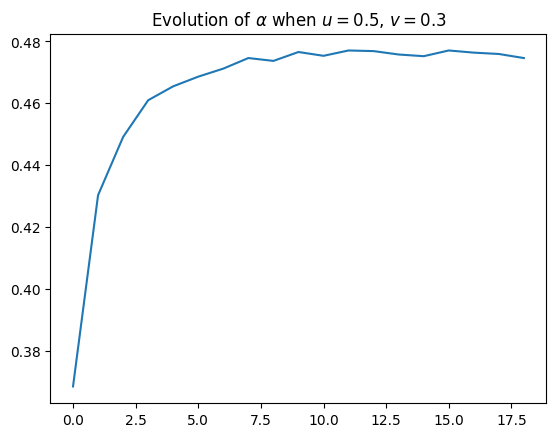
\includegraphics[width=\linewidth]{img/alpha-evolution.png}
    \caption{The evolution of $\alpha_n$}
  \end{subfigure}
  \hfill
  \begin{subfigure}[c]{0.45\linewidth}
    \centering
    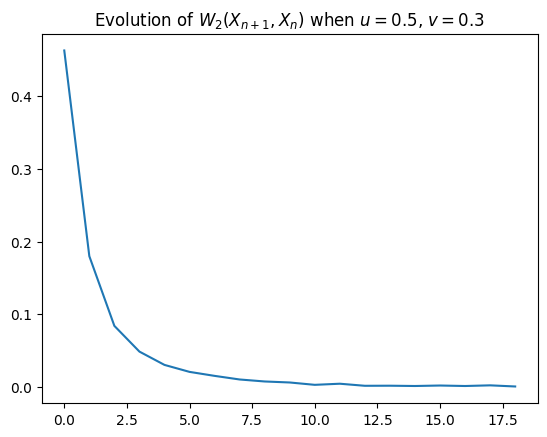
\includegraphics[width=\linewidth]{img/w2-evolution.png}
    \caption{The evolution of $W_2(\mu_{n+1}, \mu_n)$}
  \end{subfigure}

  \caption{Results of the mean-preserving recurrence \eqref{eq:mean-preserving-recurrence} with $u=0.5$ and $v=0.3$}
  \label{fig:mean-preserving-recurrence-evolution}
\end{figure}

The evolution of $\alpha$ and the 2-Wasserstein distance between consecutive distributions following the recurrence is shown in Figure \ref{fig:mean-preserving-recurrence-evolution}. Fluctuations in the final iterations are likely a side effect of the Monte Carlo simulation, since they become more stable when the number of samples is increased. However, proving that $(\mu_n, \alpha_n)$ converges may be challenging. We intended to track a quantity that evolves monotonically with the iterations. Experiments suggest in particular that the higher moments increase through iterations, but we could not complete this approach. Our alternative strategy takes advantage of Tychonoff's theorem, a non-constructive topological existence result. We summarize our proof strategy as follows, and proceed with the first step in the next subsection.
\begin{enumerate}
  \item Prove that there exists a unique solution $(X^\star, \alpha^\star)$ to \eqref{eq:limiting-equation}.
  \item Prove that for every $\epsilon > 0$, $\EE\left[Y_n/n^{\alpha^\star + \epsilon}\right]\to 0$ and $\EE\left[Y_n/n^{\alpha^\star - \epsilon}\right]\to \infty$.
  \item Prove that \eqref{eq:mean-preserving-recurrence} converges to $(X^\star, \alpha^\star)$.
\end{enumerate}

In the next subsection, we present a partial result towards the first step.

\subsection{A fixed-point approach: existence}

Since the contraction argument may not be applicable to proving uniqueness of the fixed point, we decompose the problem into proving existence and then uniqueness. Existence is proved using Tychonoff's fixed-point theorem.

\begin{theorem}[{Tychonoff \cite[Exercise 2.5c]{zeidler1986nonlinear}}]
  Let $\C$ be a nonempty, compact, convex subset of a locally convex space $\M$. Let $f: \C \to \C$ be a continuous mapping. Then $f$ has a fixed point.
\end{theorem}

We now prepare the ingredients for the Tychonoff fixed-point theorem. Ideally, the subset $\C$ should be as small as possible while still containing $(\mu_n)$ in \eqref{eq:mean-preserving-recurrence} and $(\L(X_n))$ for $X_n$ defined in \eqref{eq:scaled-recurrence} for all $\alpha\in(2u+v-1, 2u+v)$. This makes uniqueness more plausible once existence is established. Define $\Phi: \D(1) \to \D(1)$ by
\begin{equation}
  \label{eq:operator-phi}
  \Phi(\mu) = T_{\alpha(\mu)}(\mu), \quad \forall \mu\in \D(1).
\end{equation}

In the following, we will show that the subset $\C$ can be restricted to the set of distributions with uniformly bounded second moment. For $M > 0$, define
\begin{equation}
  \label{eq:bounded-second-moment}
  \D_2(1, M) = \left\{\mu\in \D(1): \int_{0}^\infty x^2 \,\mathrm{d}\mu \le M\right\}.
\end{equation}

\begin{proposition}
  \label{prop:uniform-bounded-second-moment}
  Assume that $u>1/2$. Then there exists $M_0 > 0$ such that for every $M \ge M_0 $, the operator $\Phi$ defined in \eqref{eq:operator-phi} maps $\D_2(1, M)$ into itself.
\end{proposition}


The proof is given in Appendix \ref{subsec:proof-prop-phi}. Again, the condition $u>1/2$ is crucial. Choose $M = \max(1, M_0)$. In $D_2(1,M)$, the range in Proposition \ref{prop:f} can be slightly improved to $\left[\alpha_0, 2(u+v)-1-\dfrac{v}{2M}\right)$.

The next ingredient is the host vector space $\M$. To avoid excessive elaboration, we combine two standard points of view. From probability theory, weak convergence can be defined using the space $C_b(\RR)$ of bounded, continuous test functions \cite[Chap. 1]{billingsley1999convergence}. From functional analysis, local convexity is obtained by equipping $C_b(\RR)$ with a topology and defining $\M$ as its dual space of continuous linear functionals. In this way, the weak topology on $\M$ (called the weak$^*$-topology in functional analysis) is induced by a family of seminorms $\{p_f\}_{f\in C_b(\RR)}$, which makes $\M$ a locally convex space. Finally, it is enough to have $\D_2(1, M)$ compact in $\M$. However, just as we want $\D_2(1, M)$ to be only large enough to contain our distributions of interest, we also want $\M$ to be only large enough to contain $\D_2(1, M)$, since a smaller host space is usually better behaved. We summarize the above discussion as follows, leaving the details to Appendix \ref{subsec:supp-locally-convex-spaces} and Appendix \ref{subsec:proof-prop-phi-continuity}.

\begin{theorem}[{Dual space of $C_b(\RR)$ with the strict topology \cite{buck1958bounded}}]
  \label{thm:dual-strict-topology}
  Equip $C_b(\RR)$ with the strict topology. Then the dual space is isometrically isomorphic to the space $\M(\RR)$ of bounded Radon measures on $\RR$. Moreover, $\M(\RR)$ is locally convex with respect to the weak topology.
\end{theorem}

\begin{proposition}
  \label{prop:nonempty-compact-convex}
  The set $\D_2(1, M)$ is a nonempty, compact, and convex subset of the space $\M(\RR)$ defined in Theorem \ref{thm:dual-strict-topology}.
\end{proposition}

\begin{proposition}
  \label{prop:phi-continuity}
  The operator $\Phi$ defined in \eqref{eq:operator-phi} is continuous on $\D_2(1, M)$ with respect to the weak topology.
\end{proposition}

A useful property of $\D_2(1, M)$ is that for any $\mu \in \D_2(1, M)$ and any $R > 0$, by Chebyshev's inequality, we have
$$\int_{R}^\infty x \,\mathrm{d}\mu \le \int_{R}^\infty x \left(\frac{x}{R} \right) \mathrm{d}\mu = \frac{1}{R} \int_{R}^\infty x^2 \,\mathrm{d}\mu \le \frac{1}{R} \int_{0}^\infty x^2 \,\mathrm{d}\mu \le \frac{M}{R}.$$
This implies tightness and uniform integrability of $\D_2(1, M)$. Tightness is used in proving compactness, and uniform integrability is used in proving continuity of $\Phi$ by identifying weak continuity with $W_1$-continuity.

These ingredients allow us to apply Tychonoff's fixed-point theorem.

\begin{theorem}
  \label{thm:existence-fixed-point}
  Assume that $u > 1/2$. Then there exists a solution
  $$(\mu^\star, \alpha^\star)\in \D_2(1, M)\times\left[\alpha_0, 2(u+v)-1-\dfrac{v}{2M}\right),$$
  where $\alpha_0$ solves \eqref{eq:alpha-equation}, to the fixed-point equation \eqref{eq:limiting-equation}.
\end{theorem}

% \textcolor{red}{We could construct $(\mu^\star, \alpha^\star)$. Are we really using nonconstructive topological tools somewhere?}

% \textcolor{red}{Is $\D(1)$ compact in $\M$?}



% \begin{remark}
%   If we relax the condition that the second moment is uniformly bounded.
% \end{remark}



% The problems of stronger asymptotic results remain open. Another interesting question left open is follows.

% \begin{openquestion}
%   \label{openq:alpha-algebraic}
%   Given that $y_n = n^{\alpha^\star + o(1)}$, is there an algebraic equation for $\alpha^\star$?
% \end{openquestion}

% \section{A Space of Signed Measures}
\appendix
\chapter[Appendix]{Appendix}

\section{Supplementary results}

\subsection{Asymptotics of recurrences that include a sum of history}
\label{subsec:asymptotics-of-recurrences-that-include-a-sum-of-history}

\begin{proposition}
  \label{lem:full-history-sum-asymptotics}
  Consider the sequence $(z_n)$ defined by the recurrence
  \begin{equation}
    \label{eq:full-history-sum-recurrence}
    z_{n+2} = \dfrac{K}{n}\sum\limits_{i=1}^n z_{i}, \quad n \ge 1,
  \end{equation}
  where $K > 0$. The initial values $z_1$ and $z_2$ are nonnegative and not both zero. Then $z_n\sim Cn^{K-1}$ for some constant $C > 0$.
\end{proposition}

\begin{proof}
  The recurrence is equivalent to
  $$Kz_{n+2} = \sum_{i=1}^n z_i.$$
  Let $Z(x) = \sum_{n=1}^\infty z_n x^n$ be the generating function of $(z_n)$. Summing the rewritten recurrence over $n\ge 1$ gives
  $$\sum_{n=1}^\infty n z_{n+2} x^n = K \sum_{n=1}^\infty \sum_{n=1}^\infty z_n x^n.$$

  For the left-hand side, we have
  \begin{align*}
    \sum_{n=1}^\infty n z_{n+2} x^n
     & = \frac{1}{x} \sum_{n=3}^\infty (n-2) z_n x^{n-1} = \frac{1}{x} \left( \sum_{k=3}^\infty k z_k x^{k-1} - \frac{2}{x} \sum_{k=3}^\infty z_k x^k \right) \\
     & = \frac{1}{x} \left(Z'(x) - z_1 - 2z_2 x - \frac{2}{x} \left(Z(x) - z_1 x - z_2 x^2\right) \right)                                                     \\
     & = \frac{Z'(x)}{x} - \frac{2Z(x)}{x^2} + \frac{z_1}{x}.
  \end{align*}
  For the right-hand side, we have
  $$K \sum_{n=1}^\infty \sum_{n=1}^\infty z_n x^n = K \frac{Z(x)}{1-x}.$$
  Equating the two sides and rearranging, we obtain a first-order linear differential equation
  $$Z'(x) - \left( \frac{2}{x} + \frac{Kx}{1-x} \right) Z(x) = -z_1.$$
  Multiplying both sides by the integrating factor $I(x) = x^{-2} (1-x)^K e^{Kx}$ gives
  $$[I(x) Z(x)]' = -z_1 x^{-2} (1-x)^K e^{Kx} = -z_1 x^{-2} - z_1 \frac{(1-x)^K e^{Kx} - 1}{x^2}.$$
  To integrate this from $0$ to $x$ without introducing an arbitrary integration constant, we group the singular $x^{-2}$ terms. The local expansion of $Z(x)$ at $x=0$ is $z_1 x + z_2 x^2 + \mathcal{O}(x^3)$, and the Taylor series of $(1-x)^K e^{Kx}$ begins with $1 - \frac{K}{2}x^2 + \mathcal{O}(x^3)$. Thus, we have the limit
  $$\lim_{x\to 0} \left( I(x)Z(x) - \frac{z_1}{x} \right) = \lim_{x\to 0} \left( x^{-2} (1-x)^K e^{Kx} Z(x) - \frac{z_1}{x} \right) = z_2.$$
  Furthermore, $\lim_{x\to 0} \frac{(1-x)^K e^{Kx} - 1}{x^2} = -\frac{K}{2}$, confirming that the right-hand integrand is continuous. Moving $-z_1 x^{-2}$ to the left side and integrating from $0$ to $x$ via the Fundamental Theorem of Calculus yields
  $$I(x) Z(x) - \frac{z_1}{x} - z_2 = -z_1 \int_0^x \frac{(1-t)^K e^{Kt} - 1}{t^2} \, \mathrm{d}t.$$
  Multiplying by $I(x)^{-1}$ isolates the closed-form generating function
  $$Z(x) = (1-x)^{-K} e^{-Kx} \left( z_2 x^2 + z_1 x - z_1 x^2 \int_0^x \frac{(1-t)^K e^{Kt} - 1}{t^2} \, \mathrm{d}t \right).$$
  To extract the asymptotic behavior of $(z_n)$, we analyze $Z(x)$ near its dominant singularity at $x=1$. The integral converges on $(0, 1)$, giving the local expansion
  $$Z(x) \underset{x \to 1}{\sim} A e^{-K} (1-x)^{-K},$$
  where the leading constant is
  $$A = z_2 + z_1 \left( 1 - \int_0^1 \frac{(1-t)^K e^{Kt} - 1}{t^2} \, \mathrm{d}t \right).$$
  We must ensure singularity cancellation does not occur. For any $t \in (0, 1)$, the inequality $\ln(1-t) < -t$ implies $K\ln(1-t) + Kt < 0$. Exponentiating yields $(1-t)^K e^{Kt} < 1$, so the integrand is strictly negative. Consequently, the integral evaluates to a strictly negative value, making $1 - \int_0^1 \frac{(1-t)^K e^{Kt} - 1}{t^2} \, \mathrm{d}t > 1$. Because $z_1, z_2 \ge 0$ and are not both zero, it follows that $A \ge z_2 + z_1 > 0$. Since $K > 0$, we apply Theorem \ref{thm:sim-transfer}. Mapping the $(1-x)^{-K}$ singularity to the coefficients $z_n = [x^n]Z(x)$ yields
  $$z_n \sim \frac{A e^{-K}}{\Gamma(K)} n^{K-1}.$$
  Defining $C = \frac{A e^{-K}}{\Gamma(K)}$, we have $C > 0$, completing the proof.
\end{proof}

\subsection{Spaces of probability measures}
\label{subsec:supp-locally-convex-spaces}

\begin{definition}[Weak convergence of measures]
  \label{def:weak-convergence}
  Let $(M,d)$ be a metric space and let $\M$ be the Borel $\sigma$-algebra on $M$. Let a probability distribution be defined on $(M, \M)$, and let $C_b(M)$ be the set of real-valued, bounded, continuous functions on $M$. A sequence of measures $(\mu_n)$ converges weakly to a measures $\mu$ if, for all $f\in C_b(M)$, we have
  $$\int f \, d\mu_n \to \int f \, d\mu.$$
\end{definition}

\begin{definition}[Tightness]
  \label{def:tight}
  A sequence of probability measures $(\mu_n)$ on $\RR$ is tight if for every $\varepsilon > 0$, there exists $M > 0$ such that $\sup_n \mu_n(\{x: |x| > M\}) < \varepsilon$.

  A sequence of random variables $(Z_n)$ is tight if for every $\varepsilon > 0$, there exists $M > 0$ such that $\sup_n\PP(|Z_n| > M) < \varepsilon$.
\end{definition}

\begin{theorem}[Prokhorov's theorem]
  \label{thm:prokhorov}
  A sequence of probability measures $(\mu_n)$ on $\RR$ is tight if and only if it is relatively compact in the weak topology (i.e., its closure is compact).
\end{theorem}

\section{Remaining proofs}

\subsection{Lemma \ref{lem:limiting-equation}}
\label{subsec:proof-limiting-equation}

We need the following lemma.

\begin{lemma}
  \label{lemma:average_uniform_convergence}
  Let $U_n$ be a uniform random variable on $\{1, 2, \ldots, n\}$ and let $U$ be a uniform random variable on $[0,1]$. Then $\dfrac{U_n}{n}\xlongrightarrow{d} U$.
\end{lemma}

\begin{proof}
  Recall the CDF of $U$
  $$F_U(x) = \begin{cases}
      0 & x < 0,         \\
      x & 0 \le x \le 1, \\
      1 & x > 1.
    \end{cases}$$
  Let $V_n = U_n/n$. We have $F_{V_n}(x) = \PP(U_n/n \le x) = \PP(U_n\le nx)$. Hence
  \begin{itemize}
    \item If $x\le 0$, then $F_{V_n}(x) = 0 = F_U(x)$, since $U_n\ge 1$.
    \item If $x > 1$, then $F_{V_n}(x) = 1 = F_U(x)$, since $U_n\le n$.
    \item If $0 < x \le 1$, then $F_{V_n}(x) = \dfrac{\lfloor nx \rfloor}{n}$. Since $x - \dfrac{1}{n} \le \dfrac{\lfloor nx \rfloor}{n} \le x$, we have $F_{V_n}(x) \to x = F_U(x)$.
  \end{itemize}
\end{proof}


\begin{proof}[Proof of Lemma \ref{lem:limiting-equation}]
  We first show that
  $$\left(\dfrac{U_n}{n+2}\right)^\alpha X_{U_n}^{(1)} + \left(\dfrac{n+1-U_n}{n+2}\right)^\alpha X_{n+1-U_n}^{(2)} \xlongrightarrow{d} U^\alpha X^{(1)} + (1-U)^\alpha X^{(2)}.$$

  By Lemma \ref{lemma:average_uniform_convergence} and Slutsky's theorem,
  $$\dfrac{U_n}{n+2} = \dfrac{U_n}{n} \cdot \dfrac{n}{n+2} \xlongrightarrow{d} U.$$

  To apply the Continuous Mapping Theorem, we need to show that
  $$\left(\dfrac{U_n}{n+2}, X_{U_n}^{(1)}, X_{n+1-U_n}^{(2)}\right) \xlongrightarrow{d} \left(U, X^{(1)}, X^{(2)}\right).$$

  Since $U, X^{(1)}, X^{(2)}$ are independent, this is equivalent to showing that $\forall u, x_1, x_2 \in \mathbb{R}$
  $$\PP\left(U_n \le \lfloor nu \rfloor, X_{U_n}^{(1)} \le x_1, X_{n+1-U_n}^{(2)} \le x_2\right) \longrightarrow \PP(U \le u) \PP(X^{(1)} \le x_1) \PP(X^{(2)} \le x_2).$$

  Indeed,
  \begin{align*}
     & \PP\left(U_n \le \lfloor nu \rfloor, X_{U_n}^{(1)} \le x_1, X_{n+1-U_n}^{(2)} \le x_2\right)                                                                         \\
     & = \sum_{k=1}^{\lfloor nu \rfloor} \PP(U_n=k) \PP\left(X_{k}^{(1)} \le x_1, X_{n+1-k}^{(2)} \le x_2 | U_n=k\right)                                                    \\
     & =  \dfrac{1}{n}\sum_{k=1}^{\lfloor nu \rfloor} \PP\left(X_{k}^{(1)} \le x_1, X_{n+1-k}^{(2)} \le x_2\right)               & (U_n\bot (X_{k}^{(1)}, X_{n+1-k}^{(2)})) \\
     & =  \dfrac{1}{n}\sum_{k=1}^{\lfloor nu \rfloor} \PP\left(X_{k}^{(1)} \le x_1\right)\PP\left(X_{n+1-k}^{(2)} \le x_2\right) & (X_{k}^{(1)} \bot X_{n+1-k}^{(2)})       \\
  \end{align*}

  Let $F_n$ be the common CDF of $X_n^{(1)}$ and $X_n^{(2)}$, and $F$ be the CDF of $X^{(1)}$. Let $m = \lfloor nu \rfloor$. The problem becomes showing that
  $$\dfrac{1}{n}\sum_{k=1}^{m} F_k(x_1)F_{n+1-k}(x_2) \longrightarrow u F(x_1) F(x_2).$$
  Equivalently,
  $$\dfrac{m}{n}\left(\dfrac{1}{m}\sum_{k=1}^{m} \left(F_k(x_1)F_{n+1-k}(x_2)-F(x_1) F(x_2)\right)\right) \longrightarrow 0.$$

  We have
  \begin{align*}
     & \dfrac{1}{m}\sum_{k=1}^{m} \left|F_k(x_1)F_{n+1-k}(x_2)-F(x_1) F(x_2)\right|                                                                                                       \\
     & \le \dfrac{1}{m}\sum_{k=1}^{m} \left|F_k(x_1)\left(F_{n+1-k}(x_2)-F(x_2)\right)\right| + \dfrac{1}{m}\sum_{k=1}^{m} \left|F(x_2)\left(F_k(x_1)-F(x_1)\right)\right|                \\
     & \le \dfrac{1}{m}\sum_{k=1}^{m} \left|F_{n+1-k}(x_2)-F(x_2)\right| + \dfrac{1}{m}\sum_{k=1}^{m} \left|F_k(x_1)-F(x_1)\right|                                         & (|F_n|\le 1) \\
  \end{align*}
  The second term goes to zero by the fact that $F_n(x_1)\to F(x_1)$ and Cesàro Means. We can write the first term as
  \begin{align*}
    \dfrac{1}{m}\sum_{k=n-m+1}^{n} \left|F_{k}(x_2)-F(x_2)\right|.
  \end{align*}

  If $u=1$, its convergence is similar to the second term. If $u<1$, then $n-m+1 \to \infty$. By pointwise convergence, $\forall \epsilon>0, \exists N, \forall n\ge N: |F_n(x_2)-F(x_2)|<\epsilon$. Hence, for $n-m+1\ge N$,
  \begin{align*}
    \dfrac{1}{m}\sum_{k=n-m+1}^{n} \left|F_{k}(x_2)-F(x_2)\right| < \epsilon.
  \end{align*}

  Using Slutsky's theorem again, we have

  $$\left(\dfrac{n+1}{n+2}, \dfrac{U_n}{n+2}, X_{U_n}^{(1)}, X_{n+1-U_n}^{(2)}\right) \xlongrightarrow{d} \left(1, U, X^{(1)}, X^{(2)}\right).$$

  Now define the function $f:\mathbb{R}^4_+\cap \left\{(t,u,x,y): t\ge u\right\} \to \mathbb{R}$ by
  $$f(t,u,x,y) = u^\alpha x + (t-u)^\alpha y.$$
  Then $f$ is continuous. The Continuous Mapping Theorem applies. The convergence
  $$\max\left(\left(\dfrac{U_n}{n+2}\right)^\alpha X_{U_n}^{(1)}, \left(\dfrac{n+1-U_n}{n+2}\right)^\alpha X_{n+1-U_n}^{(2)}\right) \xlongrightarrow{d} \max\left(U^\alpha X^{(1)}, (1-U)^\alpha X^{(2)}\right)$$

  is similar. And finally, we define the continuous function $g(i,j,u,v) = iu+jv$ on $\RR^4$ to finish the proof.
\end{proof}


\subsection{Proposition \ref{prop:f}}
\label{subsec:proof-prop-f}

\begin{proof}
  The function $f$ is strictly decreasing in $\alpha$. Next, we show that $f$ is continuous. The first term is continuous. We show that the second term is Lipschitz continuous. Let $\alpha, \alpha' \in (0,1]$ and assume without loss of generality that $\alpha > \alpha'$. We have
  \begin{align*}
     & \EE\left[\max\left(U^\alpha X^{(1)}, (1-U)^\alpha X^{(2)}\right) - \max\left(U^{\alpha'} X^{(1)}, (1-U)^{\alpha'} X^{(2)}\right)\right] \\
     & \le \EE\left[\max\left(\left|U^\alpha - U^{\alpha'}\right|X^{(1)}, \left|(1-U)^\alpha - (1-U)^{\alpha'}\right|X^{(2)}\right)\right]     \\
     & \le \EE\left[\left|U^\alpha - U^{\alpha'}\right|\right] + \EE\left[\left|(1-U)^\alpha - (1-U)^{\alpha'}\right|\right]                   \\
     & = 2\EE\left[\left|U^\alpha - U^{\alpha'}\right|\right]
     & \text{($U \stackrel{d}{=} 1-U$)}                                                                                                        \\
     & = 2\EE\left[U^{\alpha'} - U^{\alpha}\right]
     & \text{($U^\alpha\ge U^{\alpha'}, a.s.$)}                                                                                                \\
     & = \dfrac{2}{\alpha'+1} - \dfrac{2}{\alpha+1} = \dfrac{2(\alpha-\alpha')}{(\alpha+1)(\alpha'+1)}                                         \\
     & \le 2(\alpha-\alpha').
  \end{align*}

  Finally, we evaluate $f$ at the endpoints.
  $$\lim_{\alpha \to 0+} f(\mu, \alpha) = 2u+v\EE\left[\max\left(X^{(1)}, X^{(2)}\right)\right] > 2u+v > 1,$$
  $$f(1) = u + v\EE\left[\max\left(U^\alpha X^{(1)}, (1-U)^\alpha X^{(2)}\right)\right] \le u+v \le 1.$$
\end{proof}

\subsection{Proposition \ref{prop:uniform-bounded-second-moment}}
\label{subsec:proof-prop-phi}

\begin{proof}
  Let $\mu\in\D_2(1)$ have finite second moment, and let $Z\sim \mu$. Following the steps in the previous section, we have
  \begin{align*}
    \EE\left[\Phi(Z)^2\right]
     & \le \dfrac{2(u+v)}{2\alpha+1}\EE\left[Z^2\right] + 2uB(\alpha+1, \alpha+1) \\
     & < \dfrac{2(u+v)}{2(2u+v)-1}\EE\left[Z^2\right] + 2uB(2u+v, 2u+v)           \\
  \end{align*}
  Choose
  $$M_0 = 2uB(2u+v, 2u+v)\dfrac{2(2u+v)-1}{2u-1}.$$
  We have $\EE\left[\Phi(Z)^2\right] \le M$. Hence, $\Phi$ maps $\D_2(1, M)$ into itself.
\end{proof}

\subsection{Proposition \ref{prop:nonempty-compact-convex}}
\label{subsec:proof-prop-locally-convex-space}

\begin{proof}
  The set $\D_2(1, M)$ is nonempty since it contains $\delta_1$.

  For convexity, let $\mu, \nu \in \D_2(1, M)$. Then for every $\lambda \in [0,1]$, we have
  \begin{align*}
    \int_0^\infty x d(\lambda \mu + (1-\lambda)\nu)
     & = \lambda \int_0^\infty x d\mu + (1-\lambda) \int_0^\infty x d\nu = 1,       \\
    \int_0^\infty x^2 d(\lambda \mu + (1-\lambda)\nu)
     & = \lambda \int_0^\infty x^2 d\mu + (1-\lambda) \int_0^\infty x^2 d\nu \le M.
  \end{align*}

  For compactness, we use Prokhorov's theorem to reduce to proving that $\D_2(1, M)$ is tight and closed. Tightness is guaranteed by Chebyshev's inequality: for any $\mu \in \D_2(1, M)$ and any $R > 0$

  \begin{equation}
    \mu(\{x \ge R\}) \le \dfrac{1}{R^2}\int_{0}^\infty x^2 \,\mathrm{d}\mu \le \dfrac{M}{R^2}.
  \end{equation}

  For closedness, let $(\mu_n)$ be a sequence in $\D_2(1, M)$ that converges weakly to $\mu$. We show that $\mu \in \D_2(1, M)$. The boundedness of the second moment follows from a generalized Fatou's lemma \cite[Theorem 1.1]{feinberg2014fatou}
  $$\int_0^\infty x^2 \,\mathrm{d}\mu \le \liminf_{n \to \infty} \int_0^\infty x^2 \,\mathrm{d}\mu_n \le M.$$

  The function $x\mapsto x$ is uniformly integrable with respect to $\D_2(1, M)$ as follows. For any $\mu \in \D_2(1, M)$ and any $R > 0$
  $$\int_{R}^\infty x \,\mathrm{d}\mu \le \int_{R}^\infty x \left(\frac{x}{R} \right) \mathrm{d}\mu = \frac{1}{R} \int_{R}^\infty x^2 \,\mathrm{d}\mu \le \frac{1}{R} \int_{0}^\infty x^2 \,\mathrm{d}\mu \le \frac{M}{R}.$$
  which tends to 0 as $R \to \infty$. Therefore, the first moment converges \cite[Theorem 3.5]{billingsley1999convergence}
  $$\int_0^\infty x \,\mathrm{d}\mu_n \to \int_0^\infty x \,\mathrm{d}\mu.$$
\end{proof}

\subsection{Proposition \ref{prop:phi-continuity}}
\label{subsec:proof-prop-phi-continuity}

\begin{lemma}
  \label{lem:collapse-one-step}
  For every $\mu,\nu\in \D_2(1)$ and $\alpha\in(0,1]$, we have
  $$d_2(T_\alpha(\mu), T_\alpha(\nu)) \le \sqrt{\dfrac{2(u+v)}{2\alpha+1}}d_2(\mu, \nu) \text{ and } d_1(T_\alpha(\mu), T_\alpha(\nu)) \le \dfrac{2(u+v)}{\alpha+1}d_1(\mu, \nu).$$
\end{lemma}

\begin{proof}
  Since $I$ and $J$ are Bernoulli, we have $I^2 = I$ and $J^2 = J$. Also, from $I+J\le 1$, we have $IJ = 0$. Therefore, for every $X,X^{(1)},X^{(2)}\stackrel{\text{iid}}{\sim}\mu$ and $Y,Y^{(1)},Y^{(2)}\stackrel{\text{iid}}{\sim}\nu$, we have
  \begin{align*}
    d_2^2(T_\alpha(\mu), T_\alpha(\nu))
     & \le \EE\left[I\left(\left(U^\alpha\left(X^{(1)}-Y^{(1)}\right) + \left(1-U\right)^\alpha\left(X^{(2)}-Y^{(2)}\right)\right)\right)^2\right]                                                      \\
     & \,\,\,\,\,+\EE \left[J\left.\left(\max\left(U^\alpha X^{(1)}, \left(1-U\right)^\alpha X^{(2)}\right) - \max\left(U^\alpha Y^{(1)}, \left(1-U\right)^\alpha Y^{(2)}\right)\right)\right)^2\right] \\
     & := A+B.
  \end{align*}
  For the first expectation $A$, we use $\EE[X] = \EE[Y] = 1$ and get
  \begin{align*}
    A
     & = u\EE\left[U^{2\alpha}\left(X^{(1)}-Y^{(1)}\right)^2 + (1-U)^{2\alpha}\left(X^{(2)}-Y^{(2)}\right)^2 \right] \\
     & = \dfrac{2u}{2\alpha+1}\EE[(X-Y)^2].
  \end{align*}
  For the second one, $B$, we use the inequality
  $$(\max(a,b) - \max(c,d))^2 \le \max(a-c, b-d)^2 \le (a-c)^2+(b-d)^2$$
  for real numbers $a,b,c,d$ and get
  \begin{align*}
    B
     & \le v\EE\left[U^{2\alpha}\left(X^{(1)}-Y^{(1)}\right)^2 + (1-U)^{2\alpha}\left(X^{(2)}-Y^{(2)}\right)^2 \right] \\
     & = \dfrac{2v}{2\alpha+1}\EE[(X-Y)^2].
  \end{align*}
  Therefore,
  $$d_2^2(T_\alpha(\mu), T_\alpha(\nu)) \le \dfrac{2(u+v)}{2\alpha+1}\EE[(X-Y)^2].$$
  Taking the expectation over $X\sim\mu$ and $Y\sim\nu$, we get the desired result. The case for $d_1$ is similar.
\end{proof}

\begin{proof}[Proof of Proposition \ref{prop:phi-continuity}]
  Let $(\mu_n)$ be a sequence in $\D_2(1, M)$ that converges weakly to $\mu$, which is equivalent to $d_1(\mu_n, \mu) \to 0$. To show that $\Phi(\mu_n)\stackrel{w}{\longrightarrow}\Phi(\mu)$, we will show that $d_1(\Phi(\mu_n), \Phi(\mu)) \to 0$ by showing that $\Phi$ is Lipschitz with respect to $d_1$. Let $\mu, \nu \in \D_2(1, M)$. Write $\alpha_1 := \alpha(\mu)$ and $\alpha_2 := \alpha(\nu)$. Without loss of generality, assume that $\alpha_1 > \alpha_2$. We have
  \begin{align*}
    d_1(\Phi(\mu), \Phi(\nu))
     & = d_1(T_{\alpha_1}(\mu), T_{\alpha_2}(\nu))                                                \\
     & \le d_1(T_{\alpha_2}(\mu), T_{\alpha_2}(\nu)) + d_1(T_{\alpha_1}(\mu), T_{\alpha_2}(\mu)).
  \end{align*}
  By Lemma~\ref{lem:collapse-one-step}, we have
  $$d_1(T_{\alpha_2}(\mu), T_{\alpha_2}(\nu)) \le \dfrac{2(u+v)}{\alpha_2+1}d_1(\mu, \nu) \le 2(u+v) d_1(\mu, \nu).$$
  For the second distance, we let $Y^{(1)},Y^{(2)} \sim \nu$. Then, following the same steps as in Lemma~\ref{prop:f}, we have
  \begin{align*}
    d_1(T_{\alpha_1}(\mu), T_{\alpha_2}(\mu))
     & \le 2(u+v)(\alpha_1 - \alpha_2).
  \end{align*}
  We have $f(\mu, \alpha_1) = f(\nu, \alpha_2) = 1$. Hence
  $$|f(\mu, \alpha_1) - f(\mu, \alpha_2)| = |f(\mu, \alpha_2) - f(\nu, \alpha_2)|.$$
  Consider the left-hand side term where we fix the distribution $\mu$. We rewrite $f$ as
  $$f(\mu, \alpha) = \dfrac{2u}{\alpha+1} + v\EE\left[U^\alpha Z^{(1)}\bm{1}_{A} + (1-U)^\alpha Z^{(2)}\bm{1}_{A^c}\right], \quad Z^{(1)}, Z^{(2)} \stackrel{\text{iid}}{\sim} \mu,$$
  where $A$ is the event that $U^\alpha Z^{(1)} \ge (1-U)^\alpha Z^{(2)}$. Since $\PP\left(U^\alpha Z^{(1)} = (1-U)^\alpha Z^{(2)}\right) = 0$, we have
  \begin{align*}
    \dfrac{\partial}{\partial \alpha} f(\mu, \alpha)
     & = -\dfrac{2u}{(\alpha+1)^2} + v\EE\left[\ln(U) U^\alpha Z^{(1)} \mathbf{1}_A + \ln(1-U) (1-U)^\alpha Z^{(2)} \mathbf{1}_{A^c}\right].
  \end{align*}
  Since $\ln(U) < 0$ and $\ln(1-U) < 0$, we have for every $\alpha\in(0,1]$,
  $$\left|\dfrac{\partial}{\partial \alpha} f(\mu, \alpha)\right| \ge \dfrac{2u}{(\alpha+1)^2}.$$
  By Mean Value Theorem, we have
  $$|f(\mu, \alpha_1) - f(\mu, \alpha_2)| \ge \dfrac{2u}{(\alpha_1+1)^2}|\alpha_1 - \alpha_2|\ge \dfrac{u}{2}|\alpha_1 - \alpha_2|$$
  We also have
  $$|f(\mu, \alpha_2) - f(\nu, \alpha_2)| \le \dfrac{2v}{\alpha_2+1}d_1(\mu, \nu) \le 2v d_1(\mu, \nu).$$
  Thus,
  $$d_1(\Phi(\mu), \Phi(\nu)) \le 2(u+v)\left(1+\dfrac{4v}{u}\right)d_1(\mu, \nu).$$
\end{proof}

\chapter[Bibliography]{Bibliography}
\defbibheading{bibliography}[]{%
  \section*{#1}%
}
\printbibliography

\end{document}